\begin{enumerate}[label=\thesection.\arabic*,ref=\thesection.\theenumi]
\numberwithin{equation}{enumi}
\numberwithin{figure}{enumi}
\numberwithin{table}{enumi}

\iffalse
\item 
\label{chapters/10/11/2/1}
\iffalse
\documentclass[journal,10pt,twocolumn]{article}
\usepackage{graphicx}
\usepackage[margin=0.5in]{geometry}
\usepackage[cmex10]{amsmath}
\usepackage{array}
\usepackage{booktabs}
\title{\textbf{Circle Assignment}}
\author{Soundarya Naru}
\date{October 2022}

\providecommand{\norm}[1]{\left\lVert#1\right\rVert}
\providecommand{\abs}[1]{\left\vert#1\right\vert}
\let\vec\mathbf
\newcommand{\myvec}[1]{\ensuremath{\begin{pmatrix}#1\end{pmatrix}}}
\newcommand{\mydet}[1]{\ensuremath{\begin{vmatrix}#1\end{vmatrix}}}
\providecommand{\brak}[1]{\ensuremath{\left(#1\right)}}
\usepackage{amsmath}
\usepackage{amssymb}
\usepackage{physics}
\usepackage{listings}
\usepackage{tabularx}

\begin{document}

\maketitle
\paragraph{\textit{Problem Statement:} \\
\fi
Draw a circle of radius 6 cm.
From a point 10 cm away from its centre, construct the pair of tangents to the circle and measure their lengths.
	\begin{figure}[!ht]
		\centering
 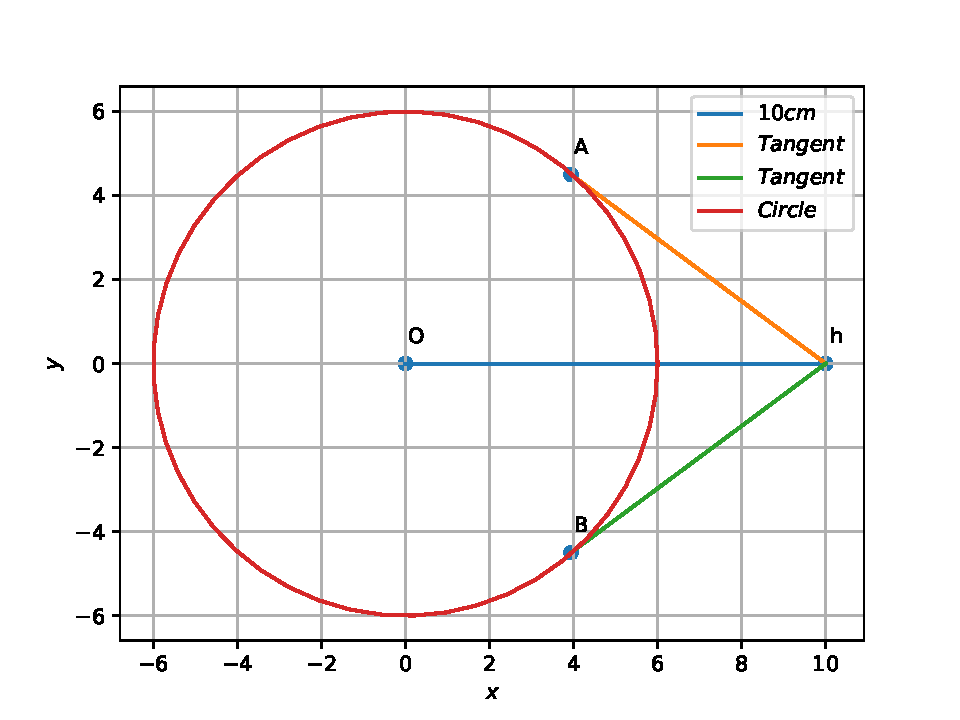
\includegraphics[width=\columnwidth]{chapters/10/11/2/1/figs/circle1.pdf}
		\caption{}
		\label{fig:10/11/2/1}
  	\end{figure}
	\\
	\solution  Follow the approach in Problem  
\ref{chapters/10/10/2/6}.
\iffalse
}

\section*{\large Solution}

\section*{\large Construction}

\begin{figure}[h]
\centering
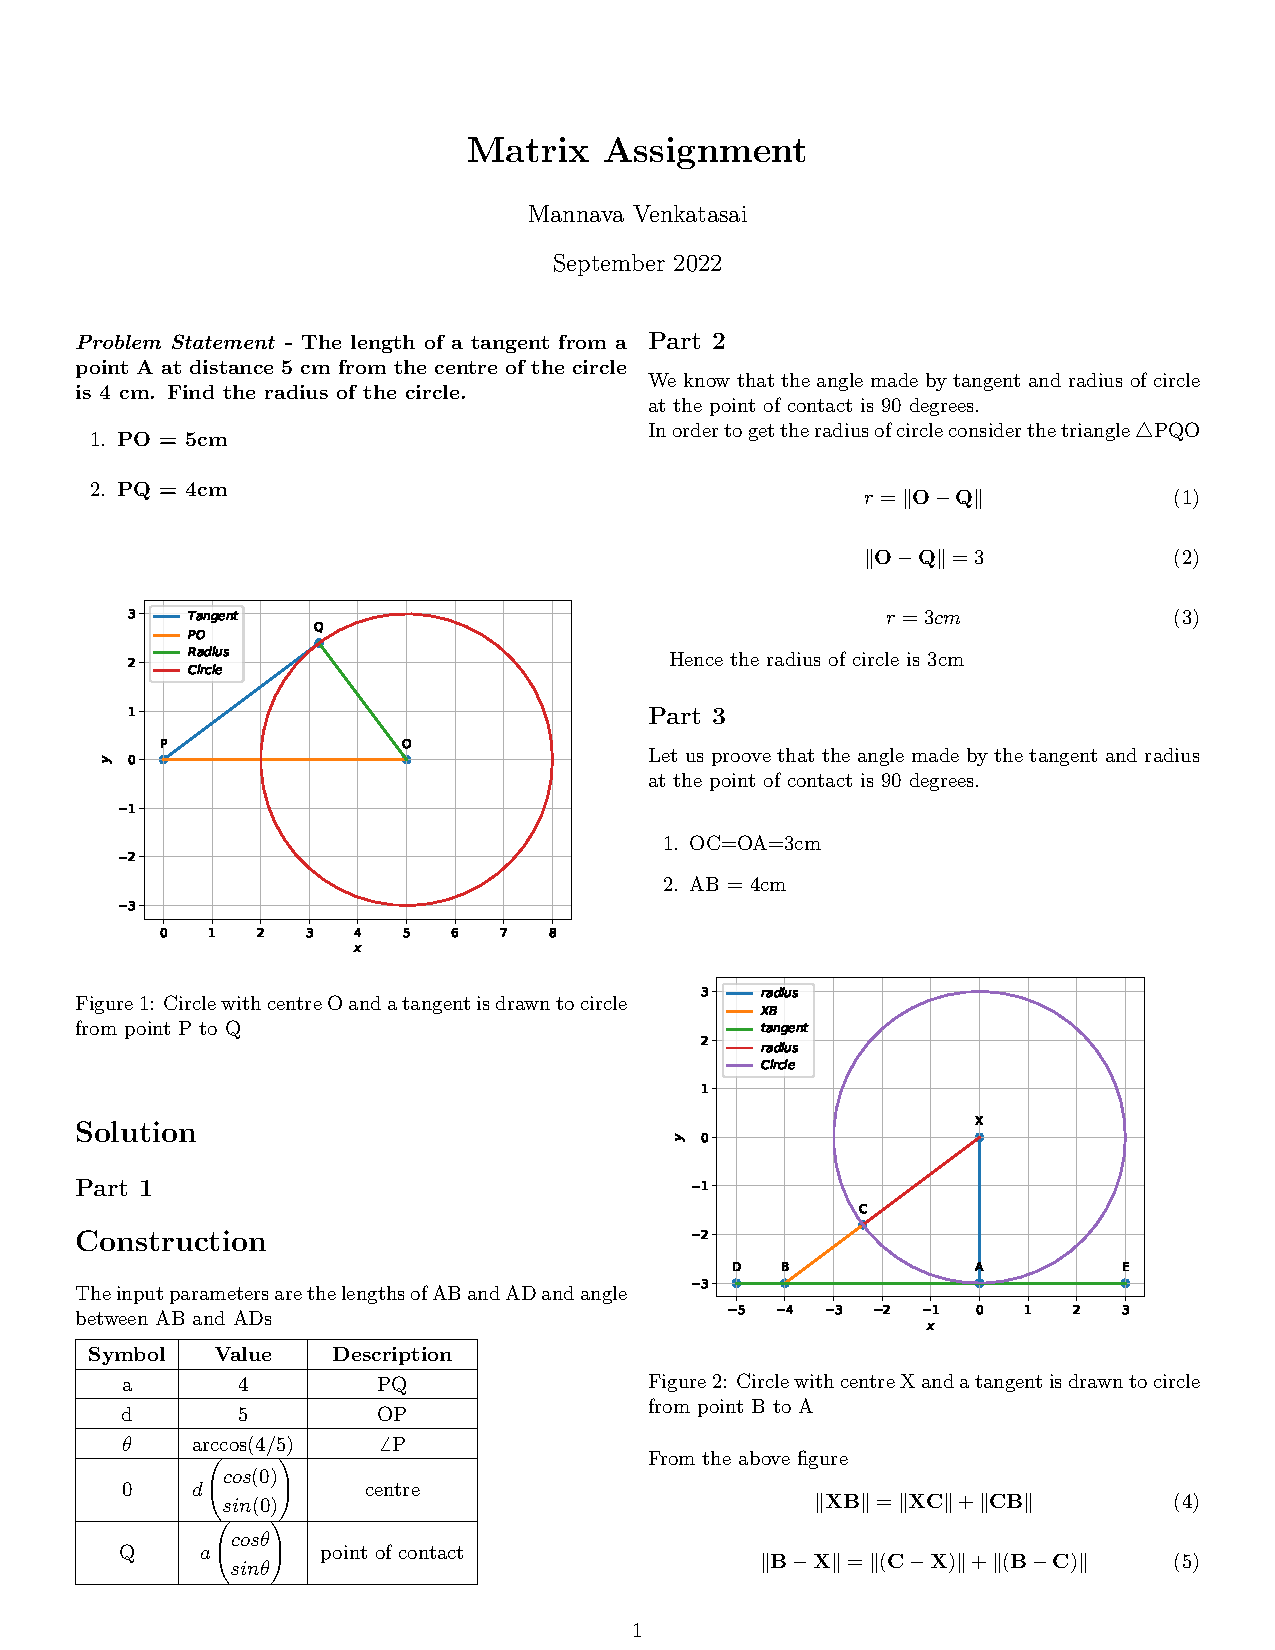
\includegraphics[width=1\columnwidth]{circle1.pdf}
\caption{Figure}
\label{fig:triangle}
\end{figure}

The dimensions of the figure is taken as below\\\\
{
\setlength\extrarowheight{2pt}
\centering
\begin{tabular}{|c|c|c|}
 \hline
 \textbf{Symbol}&\textbf{Value}&\textbf{Description}\\
 \hline
 r&6&Radius\\
 \hline
 h&10&distance\\
 \hline
 0&$d%
 \begin{pmatrix}
  cos(0)\\
  sin(0)\\
 \end{pmatrix}$%
 &centre\\
 \hline
 A&$a%
 \begin{pmatrix}
  cos\theta\\
  sin\theta\\
 \end{pmatrix}$%
 &point of contact\\
 \hline
 B&$b%
 \begin{pmatrix}
  cos\theta\\
  sin\theta\\
 \end{pmatrix}$%
 &point of contact\\
 \hline
\end{tabular}
}	
\\\\
	The equation of a conic with directrix $\vec{n^Tx}$ = c , eccentricity e anf focus $\boldsymbol{f}$ is given by
	
\begin{equation}
	\vec{x}^T\vec{V}\vec{x} + 2\vec{u}^T + f = 0
\end{equation}
	for circle eccentricity e = 0 then,\\
\begin{equation}
	\vec{V} = \vec{I} = \myvec{1&0\\0&1} , \vec{u} = \myvec{0\\0} , f = -r^2
\end{equation}
Point q on conic is given by 
\begin{equation}
	\vec{q} = \vec{V}^{-1}(\vec{n} - \vec{u})
\end{equation}
where, $\vec{n}$ is the normal vectors of the tangents from a point h to the conic are given by 
\begin{equation}
	\vec{n} = \frac{\vec{e_1}}{\vec{e_1^Th}} + \mu_i(\vec{Rh})
\end{equation}
\\
where $\mu _i$ 's are given by the following equation
\begin{equation}
	\mu_i = \frac{1}{\vec{{m^TVm}}}(\vec{-m^T(Vq+u)})	
\end{equation}
	 			$ \pm \sqrt{\vec{m^T(Vq+u)}^2 - (\vec{q^TVq + 2u^T} + f)(\vec{m^TVm)})}$
\\\\
$\mu _i$ 's are obtained by substituting the following in equation 6\\\\
\begin{equation}
	\vec{m} = (\vec{Rh})  ;  \vec{u}  = \myvec{0\\0}  ;  \vec{q} = \frac{\vec{e_1}}{\vec{e_1^Th}}
\end{equation}
 $\vec{R}$ = $\myvec{0&-1\\1&0}$ 
The obtained $\mu_i$'s are substituted in equation 5 and equation 5 is substituted in equation 6 the required points on conic A and B are obtained.\\\\
Now the point A and B are formed and tangents are drawn \\\\
To find the length of point h and point A \\
\begin{center}
	The distance between h and A is $\norm{\vec{h}-\vec{A}}$\\
\end{center}
\begin{equation}
  (\vec{h}-\vec{A})(\vec{h}-\vec{A})^T=d^2
\end{equation}
\begin{center}
	By solving  equation(7) we get \\
	    distance  d=$8cm$\\
	    \begin{equation}
  (\vec{h}-\vec{A})(\vec{h}-\vec{A})^T=d^2
\end{equation}
\end{center}
\begin{center}
	By solving  equation(7) we get \\
	    distance  d=$8cm$\\
	    \begin{equation}
	    \norm{\vec{h}-\vec{A}}=8cm
	    \end{equation}=8cm
\end{center}
To find the length of point h and point B\\
\begin{center}
	The distance between h and B is $\norm{\vec{h}-\vec{B}}$\\
\end{center}
\begin{equation}
  (\vec{h}-\vec{B})(\vec{h}-\vec{B})^T=d^2
\end{equation}
\begin{center}
	By solving  equation(10) we get \\
	    distance  d=$8cm$\\
	    \begin{equation}
	    \norm{\vec{h}-\vec{B}}=8cm
	    \end{equation}
	    from equation (9) and (11)\\
	    \begin{equation}
	    \norm{\vec{h}-\vec{A}}=\norm{\vec{h}-\vec{B}}
	    \end{equation}
	    \end{center}
	    Hence,the above equation (12) we can prove that the lenght of the tangents to a circle of radius 6cm,from a point 10cm away from the centre of the circle,is 8cm.\\
	    
	    
The below python code realizes the above construction:	\\
\begin{lstlisting}
https://github.com/soundaryanaru/FWC-assignments/blob/main/Matrix/circle_assignment/code/circle.py
\end{lstlisting}
\bibliographystyle{ieeetr}
\end{document}
\fi

\item 
\label{chapters/10/11/2/1}
\iffalse
\documentclass[journal,10pt,twocolumn]{article}
\usepackage{graphicx}
\usepackage[margin=0.5in]{geometry}
\usepackage[cmex10]{amsmath}
\usepackage{array}
\usepackage{booktabs}
\title{\textbf{Circle Assignment}}
\author{Soundarya Naru}
\date{October 2022}

\providecommand{\norm}[1]{\left\lVert#1\right\rVert}
\providecommand{\abs}[1]{\left\vert#1\right\vert}
\let\vec\mathbf
\newcommand{\myvec}[1]{\ensuremath{\begin{pmatrix}#1\end{pmatrix}}}
\newcommand{\mydet}[1]{\ensuremath{\begin{vmatrix}#1\end{vmatrix}}}
\providecommand{\brak}[1]{\ensuremath{\left(#1\right)}}
\usepackage{amsmath}
\usepackage{amssymb}
\usepackage{physics}
\usepackage{listings}
\usepackage{tabularx}

\begin{document}

\maketitle
\paragraph{\textit{Problem Statement:} \\
\fi
Draw a circle of radius 6 cm.
From a point 10 cm away from its centre, construct the pair of tangents to the circle and measure their lengths.
	\begin{figure}[!ht]
		\centering
 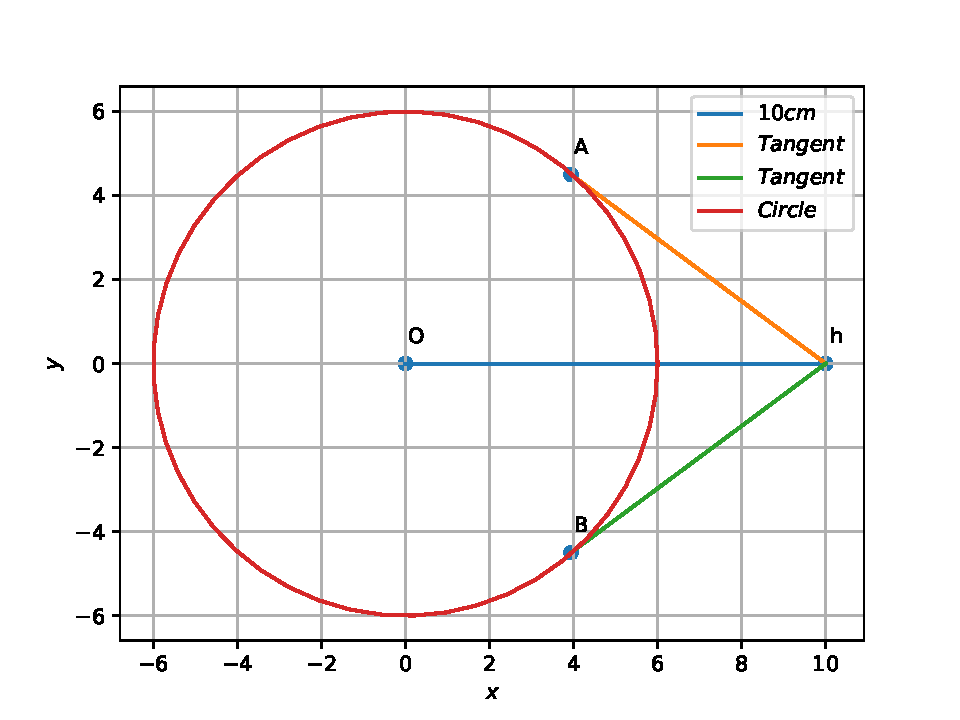
\includegraphics[width=\columnwidth]{chapters/10/11/2/1/figs/circle1.pdf}
		\caption{}
		\label{fig:10/11/2/1}
  	\end{figure}
	\\
	\solution  Follow the approach in Problem  
\ref{chapters/10/10/2/6}.
\iffalse
}

\section*{\large Solution}

\section*{\large Construction}

\begin{figure}[h]
\centering
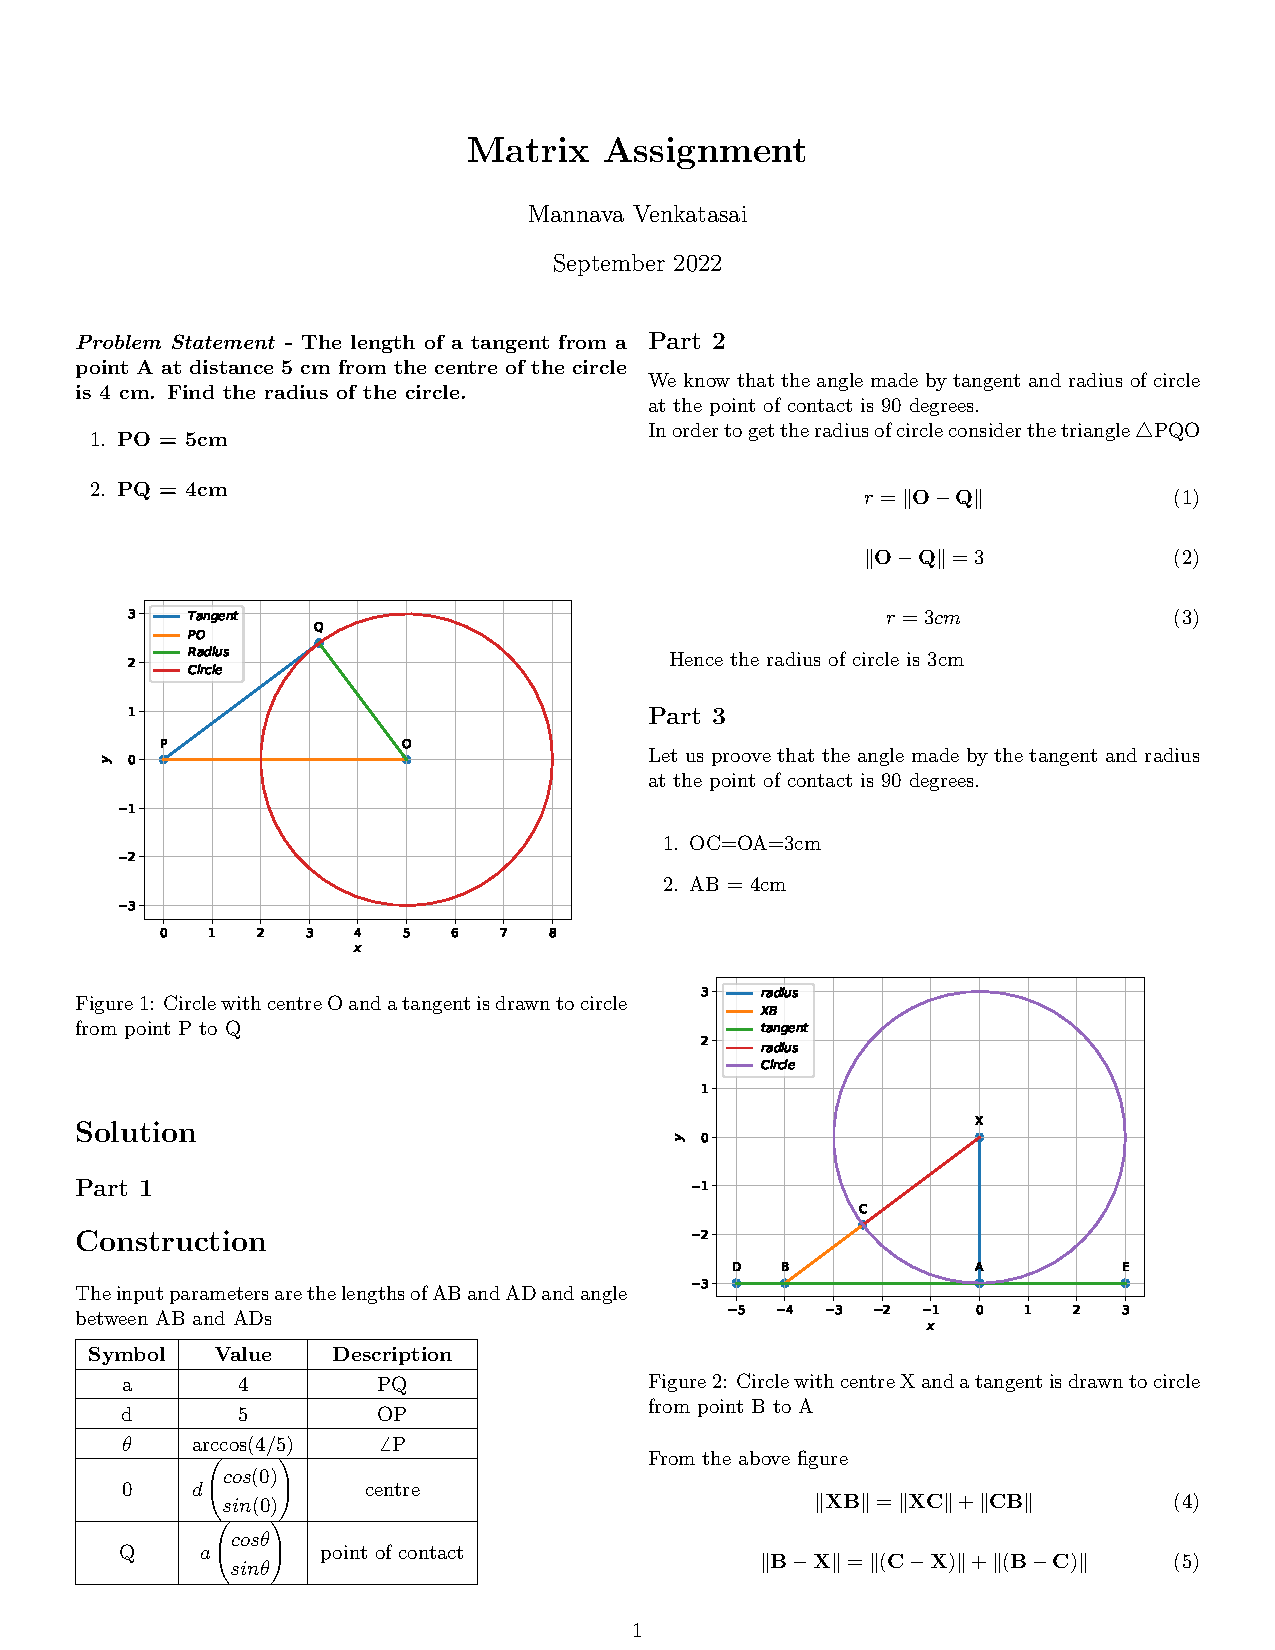
\includegraphics[width=1\columnwidth]{circle1.pdf}
\caption{Figure}
\label{fig:triangle}
\end{figure}

The dimensions of the figure is taken as below\\\\
{
\setlength\extrarowheight{2pt}
\centering
\begin{tabular}{|c|c|c|}
 \hline
 \textbf{Symbol}&\textbf{Value}&\textbf{Description}\\
 \hline
 r&6&Radius\\
 \hline
 h&10&distance\\
 \hline
 0&$d%
 \begin{pmatrix}
  cos(0)\\
  sin(0)\\
 \end{pmatrix}$%
 &centre\\
 \hline
 A&$a%
 \begin{pmatrix}
  cos\theta\\
  sin\theta\\
 \end{pmatrix}$%
 &point of contact\\
 \hline
 B&$b%
 \begin{pmatrix}
  cos\theta\\
  sin\theta\\
 \end{pmatrix}$%
 &point of contact\\
 \hline
\end{tabular}
}	
\\\\
	The equation of a conic with directrix $\vec{n^Tx}$ = c , eccentricity e anf focus $\boldsymbol{f}$ is given by
	
\begin{equation}
	\vec{x}^T\vec{V}\vec{x} + 2\vec{u}^T + f = 0
\end{equation}
	for circle eccentricity e = 0 then,\\
\begin{equation}
	\vec{V} = \vec{I} = \myvec{1&0\\0&1} , \vec{u} = \myvec{0\\0} , f = -r^2
\end{equation}
Point q on conic is given by 
\begin{equation}
	\vec{q} = \vec{V}^{-1}(\vec{n} - \vec{u})
\end{equation}
where, $\vec{n}$ is the normal vectors of the tangents from a point h to the conic are given by 
\begin{equation}
	\vec{n} = \frac{\vec{e_1}}{\vec{e_1^Th}} + \mu_i(\vec{Rh})
\end{equation}
\\
where $\mu _i$ 's are given by the following equation
\begin{equation}
	\mu_i = \frac{1}{\vec{{m^TVm}}}(\vec{-m^T(Vq+u)})	
\end{equation}
	 			$ \pm \sqrt{\vec{m^T(Vq+u)}^2 - (\vec{q^TVq + 2u^T} + f)(\vec{m^TVm)})}$
\\\\
$\mu _i$ 's are obtained by substituting the following in equation 6\\\\
\begin{equation}
	\vec{m} = (\vec{Rh})  ;  \vec{u}  = \myvec{0\\0}  ;  \vec{q} = \frac{\vec{e_1}}{\vec{e_1^Th}}
\end{equation}
 $\vec{R}$ = $\myvec{0&-1\\1&0}$ 
The obtained $\mu_i$'s are substituted in equation 5 and equation 5 is substituted in equation 6 the required points on conic A and B are obtained.\\\\
Now the point A and B are formed and tangents are drawn \\\\
To find the length of point h and point A \\
\begin{center}
	The distance between h and A is $\norm{\vec{h}-\vec{A}}$\\
\end{center}
\begin{equation}
  (\vec{h}-\vec{A})(\vec{h}-\vec{A})^T=d^2
\end{equation}
\begin{center}
	By solving  equation(7) we get \\
	    distance  d=$8cm$\\
	    \begin{equation}
  (\vec{h}-\vec{A})(\vec{h}-\vec{A})^T=d^2
\end{equation}
\end{center}
\begin{center}
	By solving  equation(7) we get \\
	    distance  d=$8cm$\\
	    \begin{equation}
	    \norm{\vec{h}-\vec{A}}=8cm
	    \end{equation}=8cm
\end{center}
To find the length of point h and point B\\
\begin{center}
	The distance between h and B is $\norm{\vec{h}-\vec{B}}$\\
\end{center}
\begin{equation}
  (\vec{h}-\vec{B})(\vec{h}-\vec{B})^T=d^2
\end{equation}
\begin{center}
	By solving  equation(10) we get \\
	    distance  d=$8cm$\\
	    \begin{equation}
	    \norm{\vec{h}-\vec{B}}=8cm
	    \end{equation}
	    from equation (9) and (11)\\
	    \begin{equation}
	    \norm{\vec{h}-\vec{A}}=\norm{\vec{h}-\vec{B}}
	    \end{equation}
	    \end{center}
	    Hence,the above equation (12) we can prove that the lenght of the tangents to a circle of radius 6cm,from a point 10cm away from the centre of the circle,is 8cm.\\
	    
	    
The below python code realizes the above construction:	\\
\begin{lstlisting}
https://github.com/soundaryanaru/FWC-assignments/blob/main/Matrix/circle_assignment/code/circle.py
\end{lstlisting}
\bibliographystyle{ieeetr}
\end{document}
\fi

\item 
\label{chapters/10/11/2/1}
\iffalse
\documentclass[journal,10pt,twocolumn]{article}
\usepackage{graphicx}
\usepackage[margin=0.5in]{geometry}
\usepackage[cmex10]{amsmath}
\usepackage{array}
\usepackage{booktabs}
\title{\textbf{Circle Assignment}}
\author{Soundarya Naru}
\date{October 2022}

\providecommand{\norm}[1]{\left\lVert#1\right\rVert}
\providecommand{\abs}[1]{\left\vert#1\right\vert}
\let\vec\mathbf
\newcommand{\myvec}[1]{\ensuremath{\begin{pmatrix}#1\end{pmatrix}}}
\newcommand{\mydet}[1]{\ensuremath{\begin{vmatrix}#1\end{vmatrix}}}
\providecommand{\brak}[1]{\ensuremath{\left(#1\right)}}
\usepackage{amsmath}
\usepackage{amssymb}
\usepackage{physics}
\usepackage{listings}
\usepackage{tabularx}

\begin{document}

\maketitle
\paragraph{\textit{Problem Statement:} \\
\fi
Draw a circle of radius 6 cm.
From a point 10 cm away from its centre, construct the pair of tangents to the circle and measure their lengths.
	\begin{figure}[!ht]
		\centering
 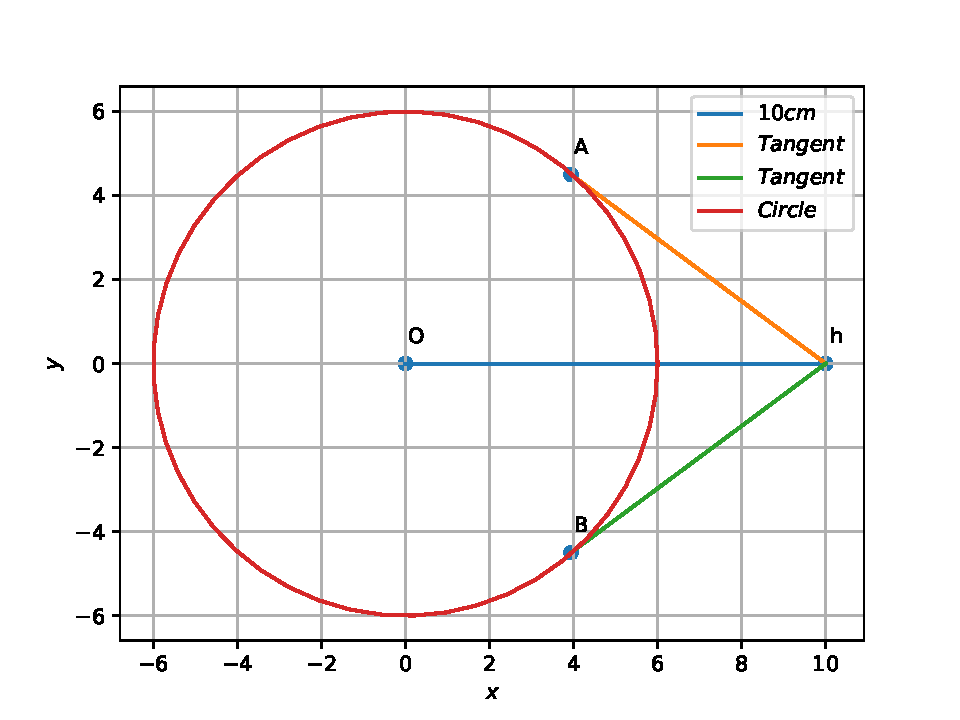
\includegraphics[width=\columnwidth]{chapters/10/11/2/1/figs/circle1.pdf}
		\caption{}
		\label{fig:10/11/2/1}
  	\end{figure}
	\\
	\solution  Follow the approach in Problem  
\ref{chapters/10/10/2/6}.
\iffalse
}

\section*{\large Solution}

\section*{\large Construction}

\begin{figure}[h]
\centering
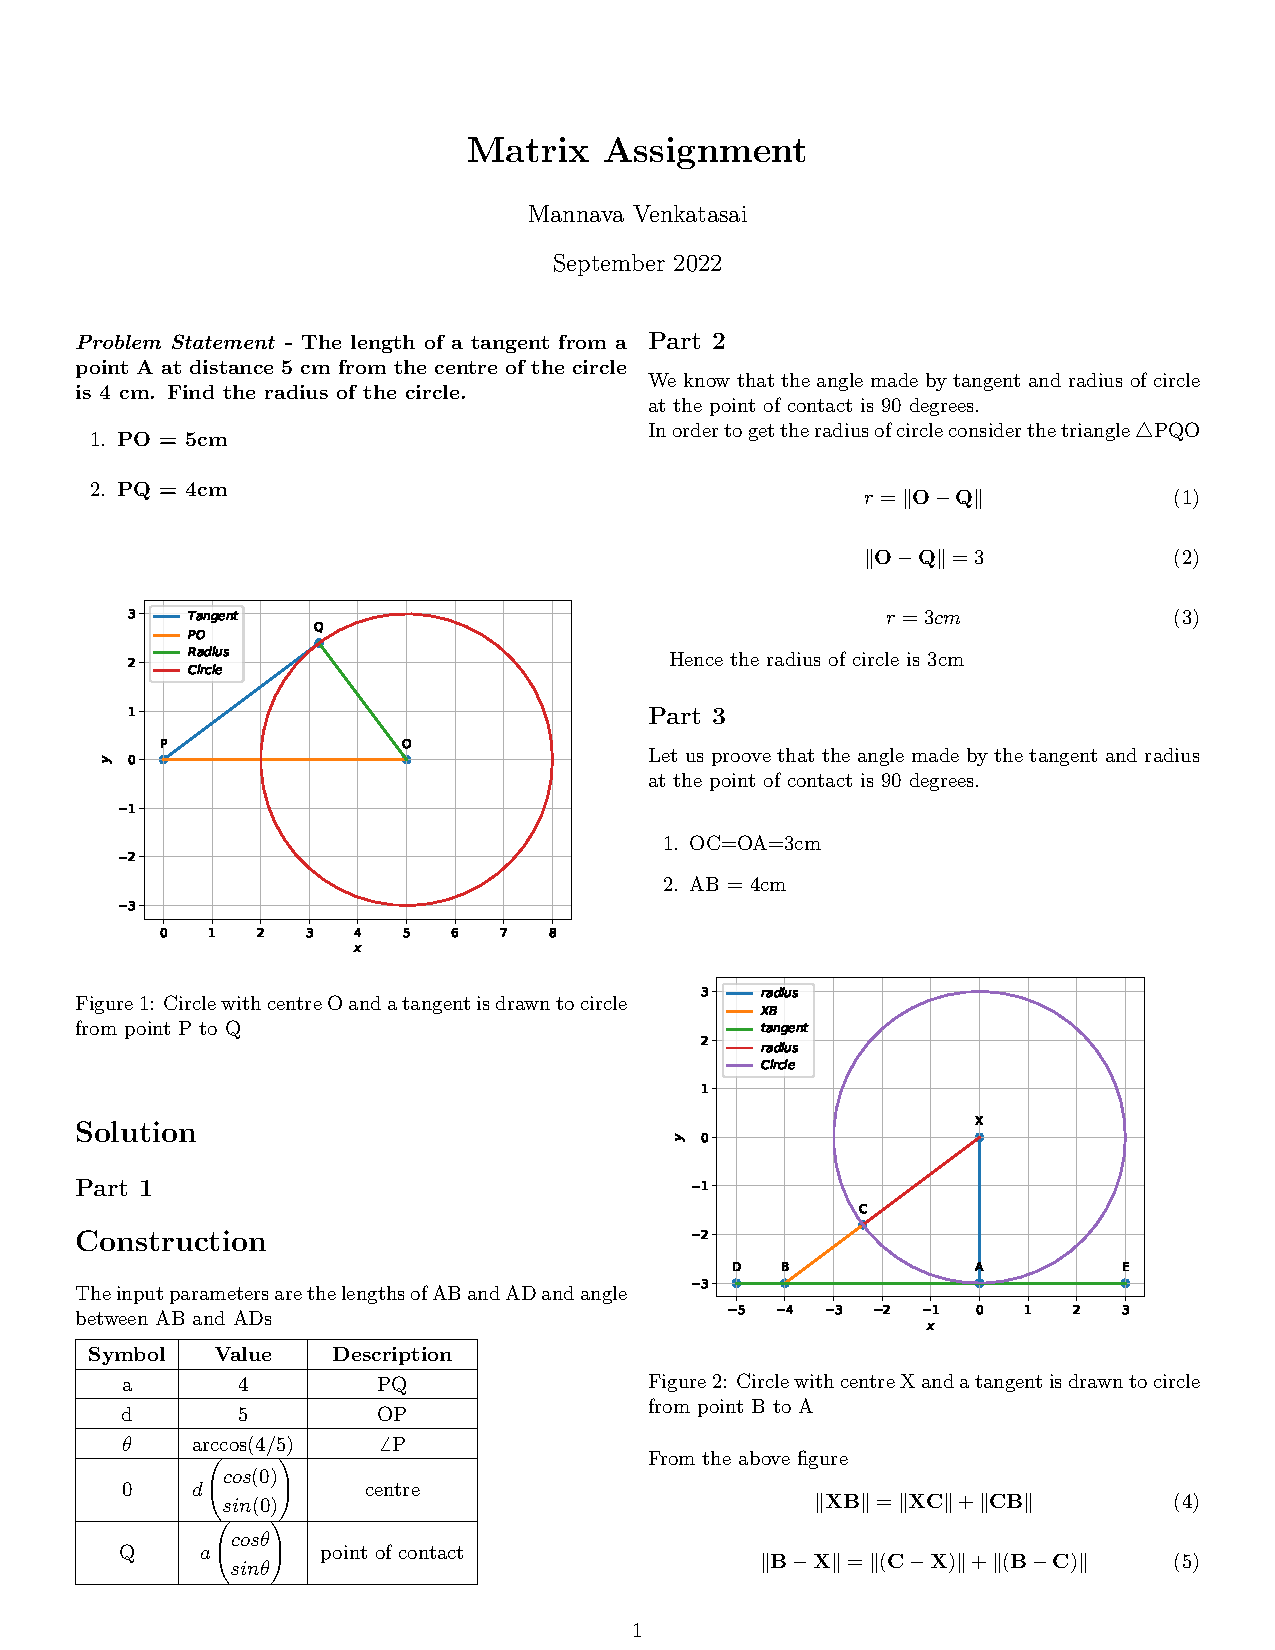
\includegraphics[width=1\columnwidth]{circle1.pdf}
\caption{Figure}
\label{fig:triangle}
\end{figure}

The dimensions of the figure is taken as below\\\\
{
\setlength\extrarowheight{2pt}
\centering
\begin{tabular}{|c|c|c|}
 \hline
 \textbf{Symbol}&\textbf{Value}&\textbf{Description}\\
 \hline
 r&6&Radius\\
 \hline
 h&10&distance\\
 \hline
 0&$d%
 \begin{pmatrix}
  cos(0)\\
  sin(0)\\
 \end{pmatrix}$%
 &centre\\
 \hline
 A&$a%
 \begin{pmatrix}
  cos\theta\\
  sin\theta\\
 \end{pmatrix}$%
 &point of contact\\
 \hline
 B&$b%
 \begin{pmatrix}
  cos\theta\\
  sin\theta\\
 \end{pmatrix}$%
 &point of contact\\
 \hline
\end{tabular}
}	
\\\\
	The equation of a conic with directrix $\vec{n^Tx}$ = c , eccentricity e anf focus $\boldsymbol{f}$ is given by
	
\begin{equation}
	\vec{x}^T\vec{V}\vec{x} + 2\vec{u}^T + f = 0
\end{equation}
	for circle eccentricity e = 0 then,\\
\begin{equation}
	\vec{V} = \vec{I} = \myvec{1&0\\0&1} , \vec{u} = \myvec{0\\0} , f = -r^2
\end{equation}
Point q on conic is given by 
\begin{equation}
	\vec{q} = \vec{V}^{-1}(\vec{n} - \vec{u})
\end{equation}
where, $\vec{n}$ is the normal vectors of the tangents from a point h to the conic are given by 
\begin{equation}
	\vec{n} = \frac{\vec{e_1}}{\vec{e_1^Th}} + \mu_i(\vec{Rh})
\end{equation}
\\
where $\mu _i$ 's are given by the following equation
\begin{equation}
	\mu_i = \frac{1}{\vec{{m^TVm}}}(\vec{-m^T(Vq+u)})	
\end{equation}
	 			$ \pm \sqrt{\vec{m^T(Vq+u)}^2 - (\vec{q^TVq + 2u^T} + f)(\vec{m^TVm)})}$
\\\\
$\mu _i$ 's are obtained by substituting the following in equation 6\\\\
\begin{equation}
	\vec{m} = (\vec{Rh})  ;  \vec{u}  = \myvec{0\\0}  ;  \vec{q} = \frac{\vec{e_1}}{\vec{e_1^Th}}
\end{equation}
 $\vec{R}$ = $\myvec{0&-1\\1&0}$ 
The obtained $\mu_i$'s are substituted in equation 5 and equation 5 is substituted in equation 6 the required points on conic A and B are obtained.\\\\
Now the point A and B are formed and tangents are drawn \\\\
To find the length of point h and point A \\
\begin{center}
	The distance between h and A is $\norm{\vec{h}-\vec{A}}$\\
\end{center}
\begin{equation}
  (\vec{h}-\vec{A})(\vec{h}-\vec{A})^T=d^2
\end{equation}
\begin{center}
	By solving  equation(7) we get \\
	    distance  d=$8cm$\\
	    \begin{equation}
  (\vec{h}-\vec{A})(\vec{h}-\vec{A})^T=d^2
\end{equation}
\end{center}
\begin{center}
	By solving  equation(7) we get \\
	    distance  d=$8cm$\\
	    \begin{equation}
	    \norm{\vec{h}-\vec{A}}=8cm
	    \end{equation}=8cm
\end{center}
To find the length of point h and point B\\
\begin{center}
	The distance between h and B is $\norm{\vec{h}-\vec{B}}$\\
\end{center}
\begin{equation}
  (\vec{h}-\vec{B})(\vec{h}-\vec{B})^T=d^2
\end{equation}
\begin{center}
	By solving  equation(10) we get \\
	    distance  d=$8cm$\\
	    \begin{equation}
	    \norm{\vec{h}-\vec{B}}=8cm
	    \end{equation}
	    from equation (9) and (11)\\
	    \begin{equation}
	    \norm{\vec{h}-\vec{A}}=\norm{\vec{h}-\vec{B}}
	    \end{equation}
	    \end{center}
	    Hence,the above equation (12) we can prove that the lenght of the tangents to a circle of radius 6cm,from a point 10cm away from the centre of the circle,is 8cm.\\
	    
	    
The below python code realizes the above construction:	\\
\begin{lstlisting}
https://github.com/soundaryanaru/FWC-assignments/blob/main/Matrix/circle_assignment/code/circle.py
\end{lstlisting}
\bibliographystyle{ieeetr}
\end{document}
\fi

\item 
\label{chapters/10/11/2/1}
\iffalse
\documentclass[journal,10pt,twocolumn]{article}
\usepackage{graphicx}
\usepackage[margin=0.5in]{geometry}
\usepackage[cmex10]{amsmath}
\usepackage{array}
\usepackage{booktabs}
\title{\textbf{Circle Assignment}}
\author{Soundarya Naru}
\date{October 2022}

\providecommand{\norm}[1]{\left\lVert#1\right\rVert}
\providecommand{\abs}[1]{\left\vert#1\right\vert}
\let\vec\mathbf
\newcommand{\myvec}[1]{\ensuremath{\begin{pmatrix}#1\end{pmatrix}}}
\newcommand{\mydet}[1]{\ensuremath{\begin{vmatrix}#1\end{vmatrix}}}
\providecommand{\brak}[1]{\ensuremath{\left(#1\right)}}
\usepackage{amsmath}
\usepackage{amssymb}
\usepackage{physics}
\usepackage{listings}
\usepackage{tabularx}

\begin{document}

\maketitle
\paragraph{\textit{Problem Statement:} \\
\fi
Draw a circle of radius 6 cm.
From a point 10 cm away from its centre, construct the pair of tangents to the circle and measure their lengths.
	\begin{figure}[!ht]
		\centering
 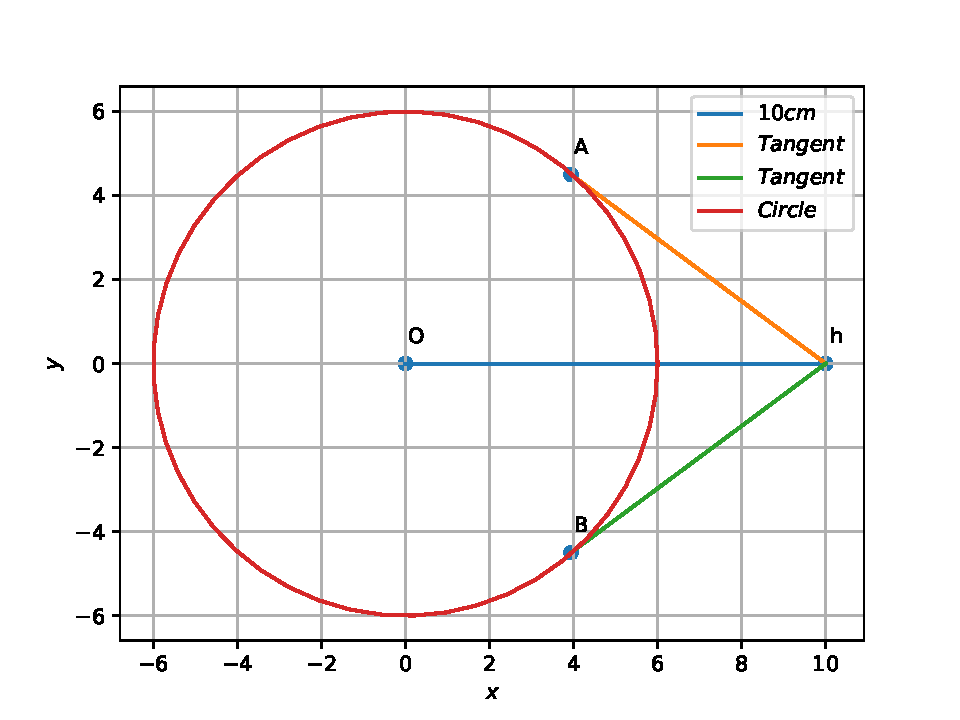
\includegraphics[width=\columnwidth]{chapters/10/11/2/1/figs/circle1.pdf}
		\caption{}
		\label{fig:10/11/2/1}
  	\end{figure}
	\\
	\solution  Follow the approach in Problem  
\ref{chapters/10/10/2/6}.
\iffalse
}

\section*{\large Solution}

\section*{\large Construction}

\begin{figure}[h]
\centering
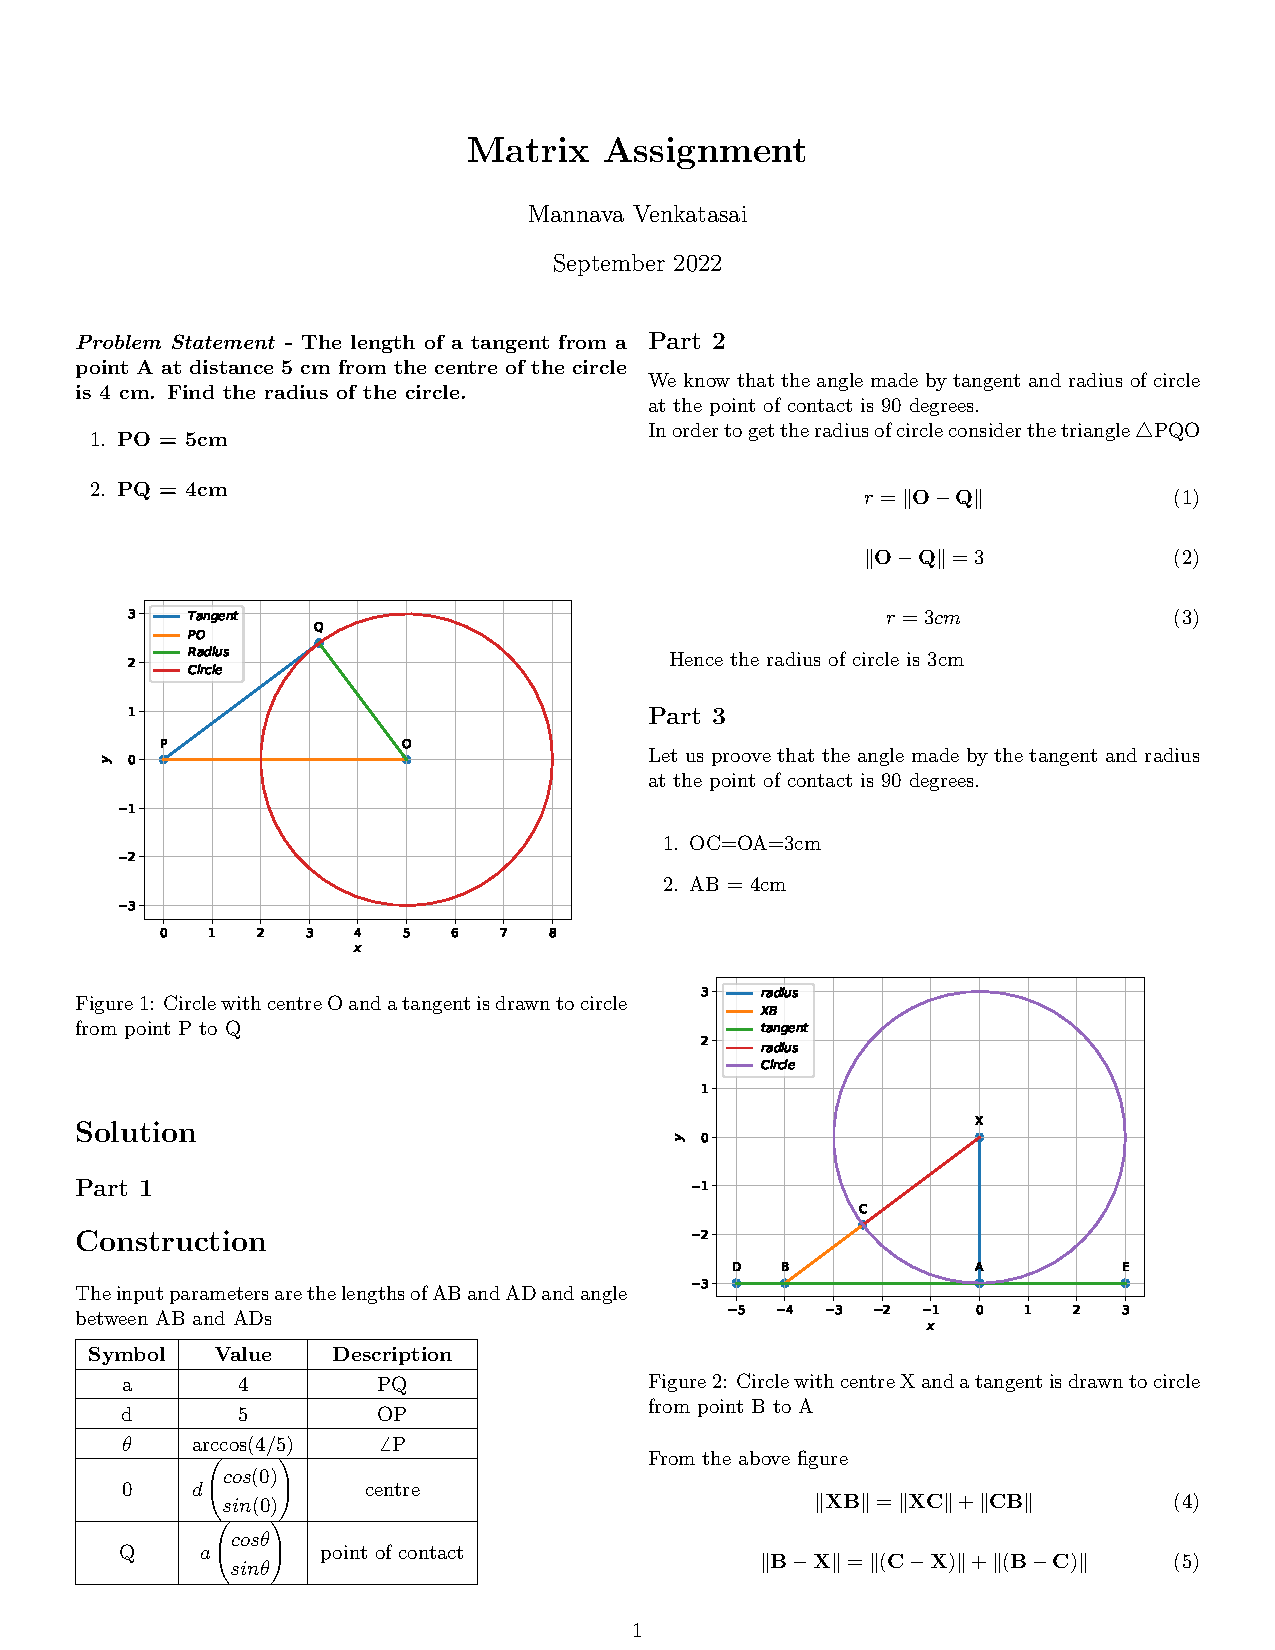
\includegraphics[width=1\columnwidth]{circle1.pdf}
\caption{Figure}
\label{fig:triangle}
\end{figure}

The dimensions of the figure is taken as below\\\\
{
\setlength\extrarowheight{2pt}
\centering
\begin{tabular}{|c|c|c|}
 \hline
 \textbf{Symbol}&\textbf{Value}&\textbf{Description}\\
 \hline
 r&6&Radius\\
 \hline
 h&10&distance\\
 \hline
 0&$d%
 \begin{pmatrix}
  cos(0)\\
  sin(0)\\
 \end{pmatrix}$%
 &centre\\
 \hline
 A&$a%
 \begin{pmatrix}
  cos\theta\\
  sin\theta\\
 \end{pmatrix}$%
 &point of contact\\
 \hline
 B&$b%
 \begin{pmatrix}
  cos\theta\\
  sin\theta\\
 \end{pmatrix}$%
 &point of contact\\
 \hline
\end{tabular}
}	
\\\\
	The equation of a conic with directrix $\vec{n^Tx}$ = c , eccentricity e anf focus $\boldsymbol{f}$ is given by
	
\begin{equation}
	\vec{x}^T\vec{V}\vec{x} + 2\vec{u}^T + f = 0
\end{equation}
	for circle eccentricity e = 0 then,\\
\begin{equation}
	\vec{V} = \vec{I} = \myvec{1&0\\0&1} , \vec{u} = \myvec{0\\0} , f = -r^2
\end{equation}
Point q on conic is given by 
\begin{equation}
	\vec{q} = \vec{V}^{-1}(\vec{n} - \vec{u})
\end{equation}
where, $\vec{n}$ is the normal vectors of the tangents from a point h to the conic are given by 
\begin{equation}
	\vec{n} = \frac{\vec{e_1}}{\vec{e_1^Th}} + \mu_i(\vec{Rh})
\end{equation}
\\
where $\mu _i$ 's are given by the following equation
\begin{equation}
	\mu_i = \frac{1}{\vec{{m^TVm}}}(\vec{-m^T(Vq+u)})	
\end{equation}
	 			$ \pm \sqrt{\vec{m^T(Vq+u)}^2 - (\vec{q^TVq + 2u^T} + f)(\vec{m^TVm)})}$
\\\\
$\mu _i$ 's are obtained by substituting the following in equation 6\\\\
\begin{equation}
	\vec{m} = (\vec{Rh})  ;  \vec{u}  = \myvec{0\\0}  ;  \vec{q} = \frac{\vec{e_1}}{\vec{e_1^Th}}
\end{equation}
 $\vec{R}$ = $\myvec{0&-1\\1&0}$ 
The obtained $\mu_i$'s are substituted in equation 5 and equation 5 is substituted in equation 6 the required points on conic A and B are obtained.\\\\
Now the point A and B are formed and tangents are drawn \\\\
To find the length of point h and point A \\
\begin{center}
	The distance between h and A is $\norm{\vec{h}-\vec{A}}$\\
\end{center}
\begin{equation}
  (\vec{h}-\vec{A})(\vec{h}-\vec{A})^T=d^2
\end{equation}
\begin{center}
	By solving  equation(7) we get \\
	    distance  d=$8cm$\\
	    \begin{equation}
  (\vec{h}-\vec{A})(\vec{h}-\vec{A})^T=d^2
\end{equation}
\end{center}
\begin{center}
	By solving  equation(7) we get \\
	    distance  d=$8cm$\\
	    \begin{equation}
	    \norm{\vec{h}-\vec{A}}=8cm
	    \end{equation}=8cm
\end{center}
To find the length of point h and point B\\
\begin{center}
	The distance between h and B is $\norm{\vec{h}-\vec{B}}$\\
\end{center}
\begin{equation}
  (\vec{h}-\vec{B})(\vec{h}-\vec{B})^T=d^2
\end{equation}
\begin{center}
	By solving  equation(10) we get \\
	    distance  d=$8cm$\\
	    \begin{equation}
	    \norm{\vec{h}-\vec{B}}=8cm
	    \end{equation}
	    from equation (9) and (11)\\
	    \begin{equation}
	    \norm{\vec{h}-\vec{A}}=\norm{\vec{h}-\vec{B}}
	    \end{equation}
	    \end{center}
	    Hence,the above equation (12) we can prove that the lenght of the tangents to a circle of radius 6cm,from a point 10cm away from the centre of the circle,is 8cm.\\
	    
	    
The below python code realizes the above construction:	\\
\begin{lstlisting}
https://github.com/soundaryanaru/FWC-assignments/blob/main/Matrix/circle_assignment/code/circle.py
\end{lstlisting}
\bibliographystyle{ieeetr}
\end{document}
\fi

\item 
\label{chapters/10/11/2/1}
\iffalse
\documentclass[journal,10pt,twocolumn]{article}
\usepackage{graphicx}
\usepackage[margin=0.5in]{geometry}
\usepackage[cmex10]{amsmath}
\usepackage{array}
\usepackage{booktabs}
\title{\textbf{Circle Assignment}}
\author{Soundarya Naru}
\date{October 2022}

\providecommand{\norm}[1]{\left\lVert#1\right\rVert}
\providecommand{\abs}[1]{\left\vert#1\right\vert}
\let\vec\mathbf
\newcommand{\myvec}[1]{\ensuremath{\begin{pmatrix}#1\end{pmatrix}}}
\newcommand{\mydet}[1]{\ensuremath{\begin{vmatrix}#1\end{vmatrix}}}
\providecommand{\brak}[1]{\ensuremath{\left(#1\right)}}
\usepackage{amsmath}
\usepackage{amssymb}
\usepackage{physics}
\usepackage{listings}
\usepackage{tabularx}

\begin{document}

\maketitle
\paragraph{\textit{Problem Statement:} \\
\fi
Draw a circle of radius 6 cm.
From a point 10 cm away from its centre, construct the pair of tangents to the circle and measure their lengths.
	\begin{figure}[!ht]
		\centering
 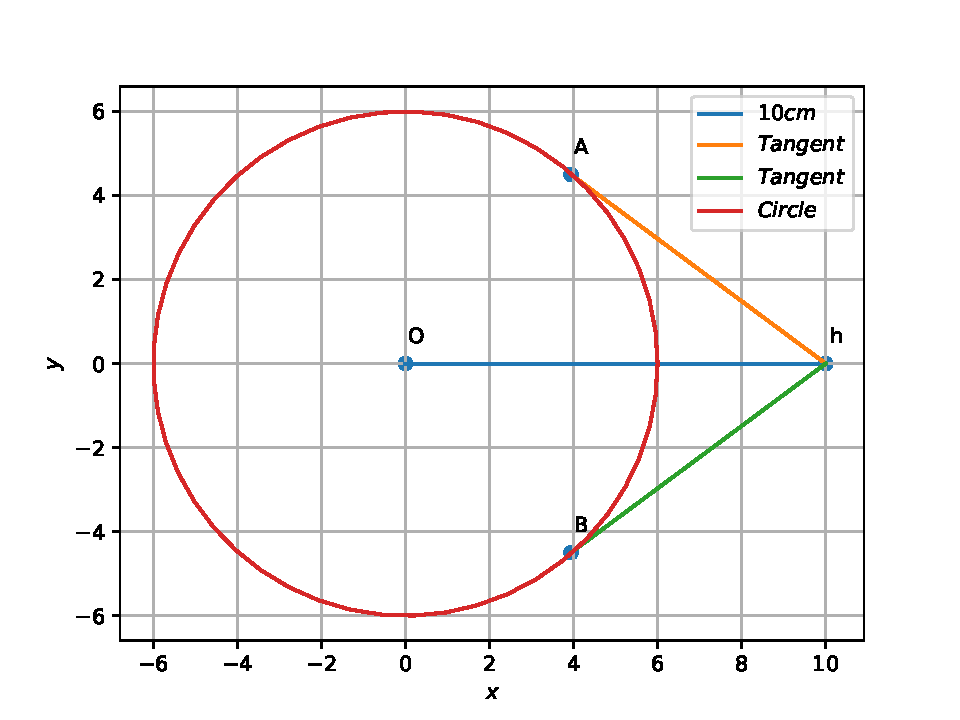
\includegraphics[width=\columnwidth]{chapters/10/11/2/1/figs/circle1.pdf}
		\caption{}
		\label{fig:10/11/2/1}
  	\end{figure}
	\\
	\solution  Follow the approach in Problem  
\ref{chapters/10/10/2/6}.
\iffalse
}

\section*{\large Solution}

\section*{\large Construction}

\begin{figure}[h]
\centering
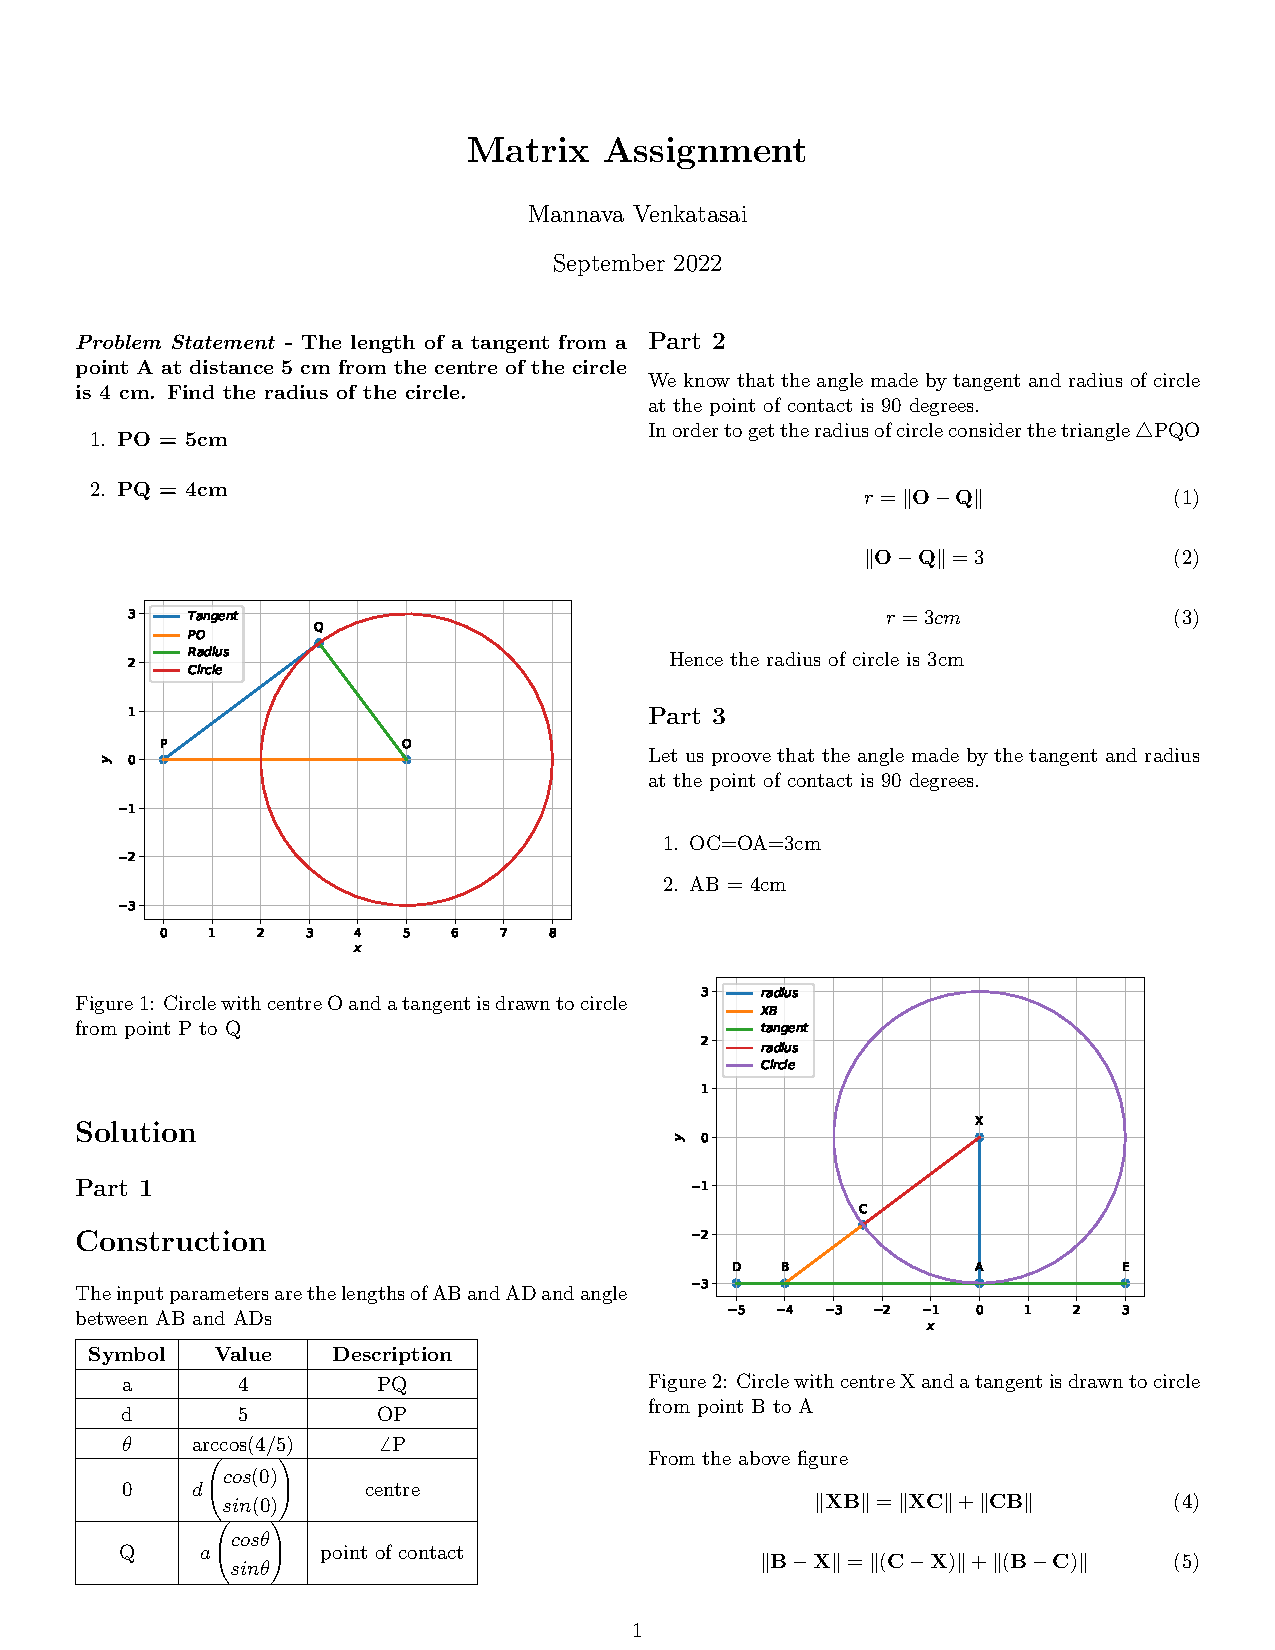
\includegraphics[width=1\columnwidth]{circle1.pdf}
\caption{Figure}
\label{fig:triangle}
\end{figure}

The dimensions of the figure is taken as below\\\\
{
\setlength\extrarowheight{2pt}
\centering
\begin{tabular}{|c|c|c|}
 \hline
 \textbf{Symbol}&\textbf{Value}&\textbf{Description}\\
 \hline
 r&6&Radius\\
 \hline
 h&10&distance\\
 \hline
 0&$d%
 \begin{pmatrix}
  cos(0)\\
  sin(0)\\
 \end{pmatrix}$%
 &centre\\
 \hline
 A&$a%
 \begin{pmatrix}
  cos\theta\\
  sin\theta\\
 \end{pmatrix}$%
 &point of contact\\
 \hline
 B&$b%
 \begin{pmatrix}
  cos\theta\\
  sin\theta\\
 \end{pmatrix}$%
 &point of contact\\
 \hline
\end{tabular}
}	
\\\\
	The equation of a conic with directrix $\vec{n^Tx}$ = c , eccentricity e anf focus $\boldsymbol{f}$ is given by
	
\begin{equation}
	\vec{x}^T\vec{V}\vec{x} + 2\vec{u}^T + f = 0
\end{equation}
	for circle eccentricity e = 0 then,\\
\begin{equation}
	\vec{V} = \vec{I} = \myvec{1&0\\0&1} , \vec{u} = \myvec{0\\0} , f = -r^2
\end{equation}
Point q on conic is given by 
\begin{equation}
	\vec{q} = \vec{V}^{-1}(\vec{n} - \vec{u})
\end{equation}
where, $\vec{n}$ is the normal vectors of the tangents from a point h to the conic are given by 
\begin{equation}
	\vec{n} = \frac{\vec{e_1}}{\vec{e_1^Th}} + \mu_i(\vec{Rh})
\end{equation}
\\
where $\mu _i$ 's are given by the following equation
\begin{equation}
	\mu_i = \frac{1}{\vec{{m^TVm}}}(\vec{-m^T(Vq+u)})	
\end{equation}
	 			$ \pm \sqrt{\vec{m^T(Vq+u)}^2 - (\vec{q^TVq + 2u^T} + f)(\vec{m^TVm)})}$
\\\\
$\mu _i$ 's are obtained by substituting the following in equation 6\\\\
\begin{equation}
	\vec{m} = (\vec{Rh})  ;  \vec{u}  = \myvec{0\\0}  ;  \vec{q} = \frac{\vec{e_1}}{\vec{e_1^Th}}
\end{equation}
 $\vec{R}$ = $\myvec{0&-1\\1&0}$ 
The obtained $\mu_i$'s are substituted in equation 5 and equation 5 is substituted in equation 6 the required points on conic A and B are obtained.\\\\
Now the point A and B are formed and tangents are drawn \\\\
To find the length of point h and point A \\
\begin{center}
	The distance between h and A is $\norm{\vec{h}-\vec{A}}$\\
\end{center}
\begin{equation}
  (\vec{h}-\vec{A})(\vec{h}-\vec{A})^T=d^2
\end{equation}
\begin{center}
	By solving  equation(7) we get \\
	    distance  d=$8cm$\\
	    \begin{equation}
  (\vec{h}-\vec{A})(\vec{h}-\vec{A})^T=d^2
\end{equation}
\end{center}
\begin{center}
	By solving  equation(7) we get \\
	    distance  d=$8cm$\\
	    \begin{equation}
	    \norm{\vec{h}-\vec{A}}=8cm
	    \end{equation}=8cm
\end{center}
To find the length of point h and point B\\
\begin{center}
	The distance between h and B is $\norm{\vec{h}-\vec{B}}$\\
\end{center}
\begin{equation}
  (\vec{h}-\vec{B})(\vec{h}-\vec{B})^T=d^2
\end{equation}
\begin{center}
	By solving  equation(10) we get \\
	    distance  d=$8cm$\\
	    \begin{equation}
	    \norm{\vec{h}-\vec{B}}=8cm
	    \end{equation}
	    from equation (9) and (11)\\
	    \begin{equation}
	    \norm{\vec{h}-\vec{A}}=\norm{\vec{h}-\vec{B}}
	    \end{equation}
	    \end{center}
	    Hence,the above equation (12) we can prove that the lenght of the tangents to a circle of radius 6cm,from a point 10cm away from the centre of the circle,is 8cm.\\
	    
	    
The below python code realizes the above construction:	\\
\begin{lstlisting}
https://github.com/soundaryanaru/FWC-assignments/blob/main/Matrix/circle_assignment/code/circle.py
\end{lstlisting}
\bibliographystyle{ieeetr}
\end{document}
\fi

\item 
\label{chapters/10/11/2/1}
\iffalse
\documentclass[journal,10pt,twocolumn]{article}
\usepackage{graphicx}
\usepackage[margin=0.5in]{geometry}
\usepackage[cmex10]{amsmath}
\usepackage{array}
\usepackage{booktabs}
\title{\textbf{Circle Assignment}}
\author{Soundarya Naru}
\date{October 2022}

\providecommand{\norm}[1]{\left\lVert#1\right\rVert}
\providecommand{\abs}[1]{\left\vert#1\right\vert}
\let\vec\mathbf
\newcommand{\myvec}[1]{\ensuremath{\begin{pmatrix}#1\end{pmatrix}}}
\newcommand{\mydet}[1]{\ensuremath{\begin{vmatrix}#1\end{vmatrix}}}
\providecommand{\brak}[1]{\ensuremath{\left(#1\right)}}
\usepackage{amsmath}
\usepackage{amssymb}
\usepackage{physics}
\usepackage{listings}
\usepackage{tabularx}

\begin{document}

\maketitle
\paragraph{\textit{Problem Statement:} \\
\fi
Draw a circle of radius 6 cm.
From a point 10 cm away from its centre, construct the pair of tangents to the circle and measure their lengths.
	\begin{figure}[!ht]
		\centering
 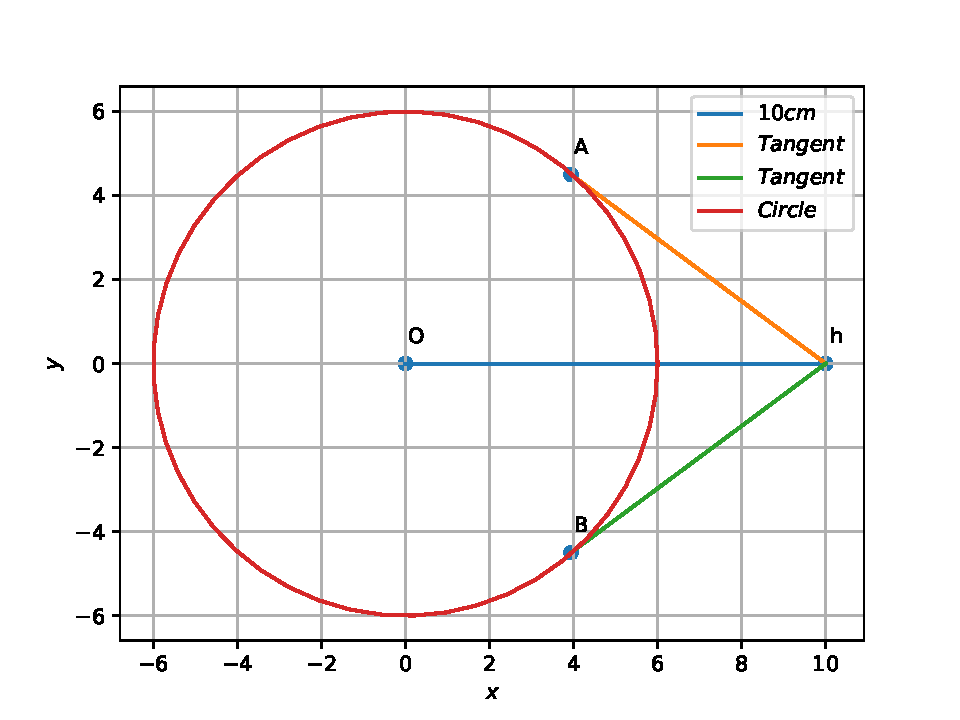
\includegraphics[width=\columnwidth]{chapters/10/11/2/1/figs/circle1.pdf}
		\caption{}
		\label{fig:10/11/2/1}
  	\end{figure}
	\\
	\solution  Follow the approach in Problem  
\ref{chapters/10/10/2/6}.
\iffalse
}

\section*{\large Solution}

\section*{\large Construction}

\begin{figure}[h]
\centering
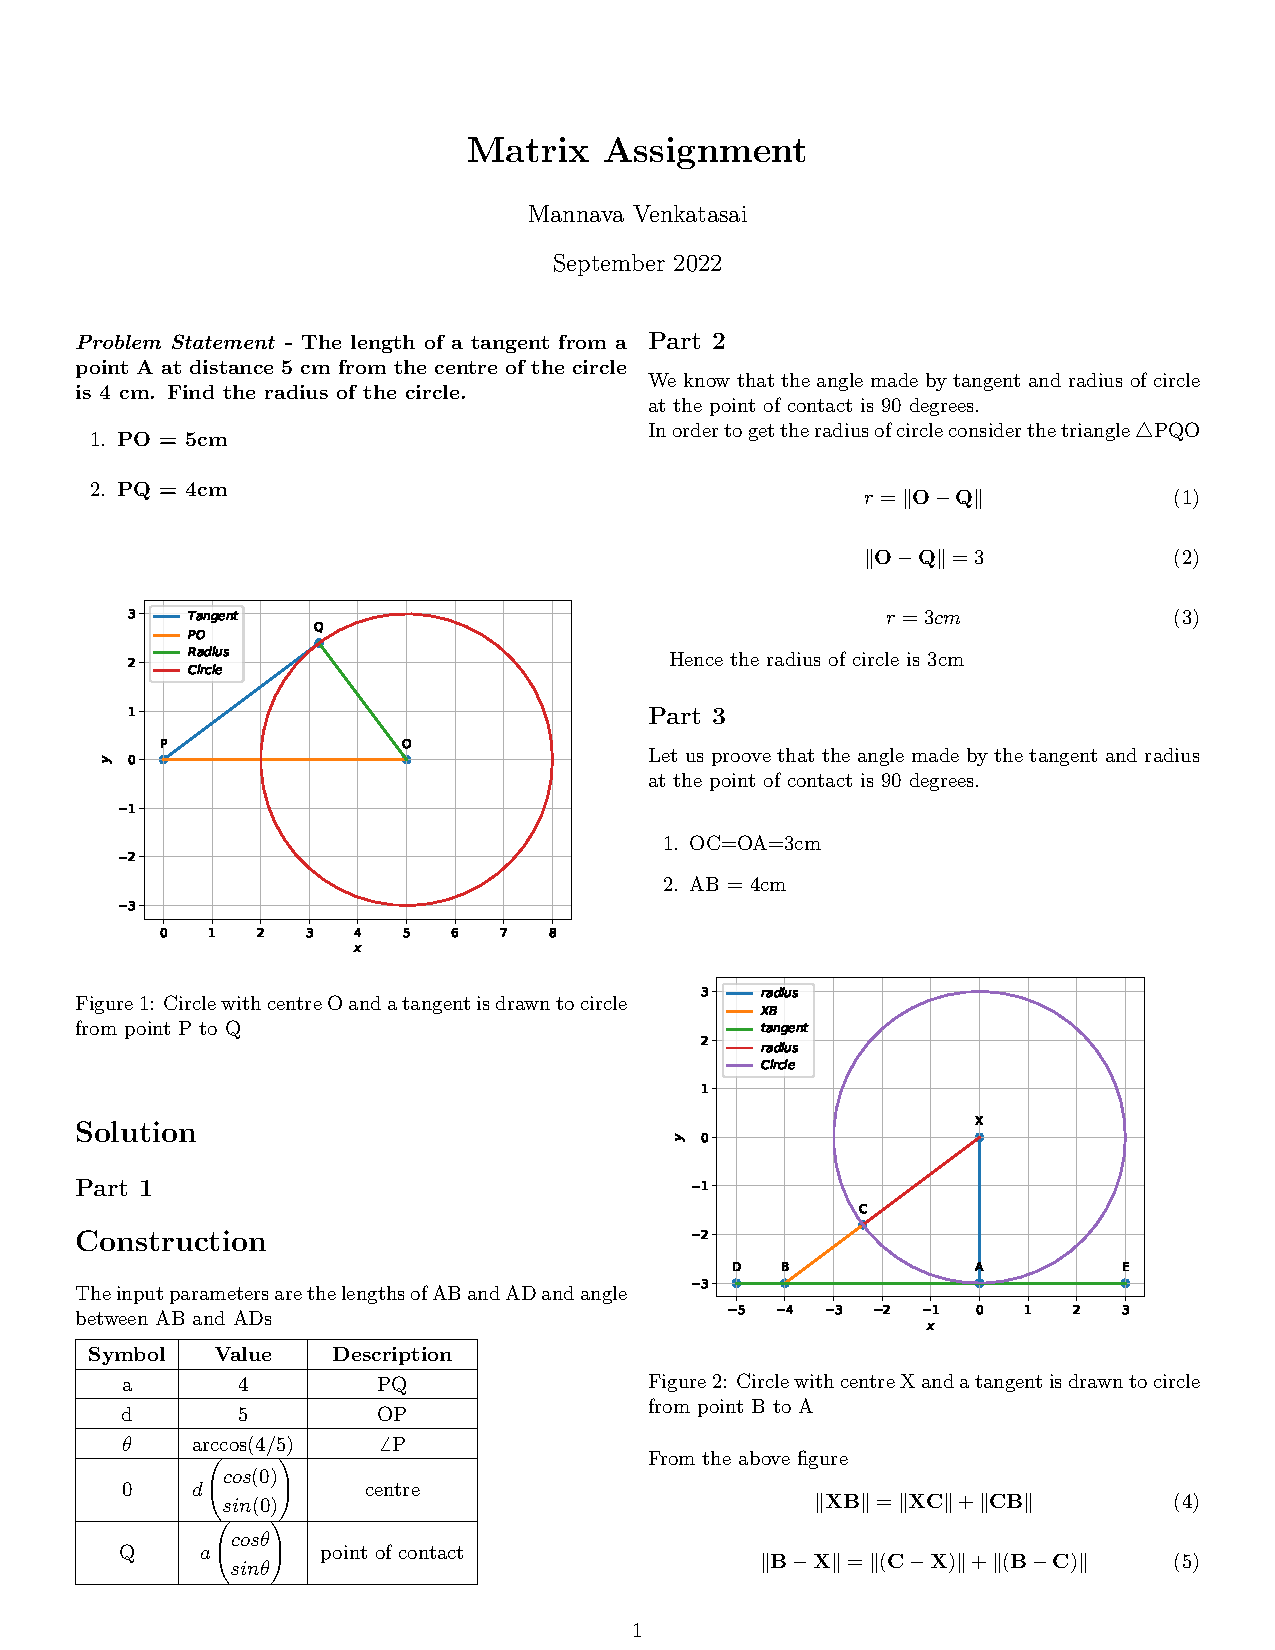
\includegraphics[width=1\columnwidth]{circle1.pdf}
\caption{Figure}
\label{fig:triangle}
\end{figure}

The dimensions of the figure is taken as below\\\\
{
\setlength\extrarowheight{2pt}
\centering
\begin{tabular}{|c|c|c|}
 \hline
 \textbf{Symbol}&\textbf{Value}&\textbf{Description}\\
 \hline
 r&6&Radius\\
 \hline
 h&10&distance\\
 \hline
 0&$d%
 \begin{pmatrix}
  cos(0)\\
  sin(0)\\
 \end{pmatrix}$%
 &centre\\
 \hline
 A&$a%
 \begin{pmatrix}
  cos\theta\\
  sin\theta\\
 \end{pmatrix}$%
 &point of contact\\
 \hline
 B&$b%
 \begin{pmatrix}
  cos\theta\\
  sin\theta\\
 \end{pmatrix}$%
 &point of contact\\
 \hline
\end{tabular}
}	
\\\\
	The equation of a conic with directrix $\vec{n^Tx}$ = c , eccentricity e anf focus $\boldsymbol{f}$ is given by
	
\begin{equation}
	\vec{x}^T\vec{V}\vec{x} + 2\vec{u}^T + f = 0
\end{equation}
	for circle eccentricity e = 0 then,\\
\begin{equation}
	\vec{V} = \vec{I} = \myvec{1&0\\0&1} , \vec{u} = \myvec{0\\0} , f = -r^2
\end{equation}
Point q on conic is given by 
\begin{equation}
	\vec{q} = \vec{V}^{-1}(\vec{n} - \vec{u})
\end{equation}
where, $\vec{n}$ is the normal vectors of the tangents from a point h to the conic are given by 
\begin{equation}
	\vec{n} = \frac{\vec{e_1}}{\vec{e_1^Th}} + \mu_i(\vec{Rh})
\end{equation}
\\
where $\mu _i$ 's are given by the following equation
\begin{equation}
	\mu_i = \frac{1}{\vec{{m^TVm}}}(\vec{-m^T(Vq+u)})	
\end{equation}
	 			$ \pm \sqrt{\vec{m^T(Vq+u)}^2 - (\vec{q^TVq + 2u^T} + f)(\vec{m^TVm)})}$
\\\\
$\mu _i$ 's are obtained by substituting the following in equation 6\\\\
\begin{equation}
	\vec{m} = (\vec{Rh})  ;  \vec{u}  = \myvec{0\\0}  ;  \vec{q} = \frac{\vec{e_1}}{\vec{e_1^Th}}
\end{equation}
 $\vec{R}$ = $\myvec{0&-1\\1&0}$ 
The obtained $\mu_i$'s are substituted in equation 5 and equation 5 is substituted in equation 6 the required points on conic A and B are obtained.\\\\
Now the point A and B are formed and tangents are drawn \\\\
To find the length of point h and point A \\
\begin{center}
	The distance between h and A is $\norm{\vec{h}-\vec{A}}$\\
\end{center}
\begin{equation}
  (\vec{h}-\vec{A})(\vec{h}-\vec{A})^T=d^2
\end{equation}
\begin{center}
	By solving  equation(7) we get \\
	    distance  d=$8cm$\\
	    \begin{equation}
  (\vec{h}-\vec{A})(\vec{h}-\vec{A})^T=d^2
\end{equation}
\end{center}
\begin{center}
	By solving  equation(7) we get \\
	    distance  d=$8cm$\\
	    \begin{equation}
	    \norm{\vec{h}-\vec{A}}=8cm
	    \end{equation}=8cm
\end{center}
To find the length of point h and point B\\
\begin{center}
	The distance between h and B is $\norm{\vec{h}-\vec{B}}$\\
\end{center}
\begin{equation}
  (\vec{h}-\vec{B})(\vec{h}-\vec{B})^T=d^2
\end{equation}
\begin{center}
	By solving  equation(10) we get \\
	    distance  d=$8cm$\\
	    \begin{equation}
	    \norm{\vec{h}-\vec{B}}=8cm
	    \end{equation}
	    from equation (9) and (11)\\
	    \begin{equation}
	    \norm{\vec{h}-\vec{A}}=\norm{\vec{h}-\vec{B}}
	    \end{equation}
	    \end{center}
	    Hence,the above equation (12) we can prove that the lenght of the tangents to a circle of radius 6cm,from a point 10cm away from the centre of the circle,is 8cm.\\
	    
	    
The below python code realizes the above construction:	\\
\begin{lstlisting}
https://github.com/soundaryanaru/FWC-assignments/blob/main/Matrix/circle_assignment/code/circle.py
\end{lstlisting}
\bibliographystyle{ieeetr}
\end{document}
\fi

\item 
\label{chapters/10/11/2/1}
\iffalse
\documentclass[journal,10pt,twocolumn]{article}
\usepackage{graphicx}
\usepackage[margin=0.5in]{geometry}
\usepackage[cmex10]{amsmath}
\usepackage{array}
\usepackage{booktabs}
\title{\textbf{Circle Assignment}}
\author{Soundarya Naru}
\date{October 2022}

\providecommand{\norm}[1]{\left\lVert#1\right\rVert}
\providecommand{\abs}[1]{\left\vert#1\right\vert}
\let\vec\mathbf
\newcommand{\myvec}[1]{\ensuremath{\begin{pmatrix}#1\end{pmatrix}}}
\newcommand{\mydet}[1]{\ensuremath{\begin{vmatrix}#1\end{vmatrix}}}
\providecommand{\brak}[1]{\ensuremath{\left(#1\right)}}
\usepackage{amsmath}
\usepackage{amssymb}
\usepackage{physics}
\usepackage{listings}
\usepackage{tabularx}

\begin{document}

\maketitle
\paragraph{\textit{Problem Statement:} \\
\fi
Draw a circle of radius 6 cm.
From a point 10 cm away from its centre, construct the pair of tangents to the circle and measure their lengths.
	\begin{figure}[!ht]
		\centering
 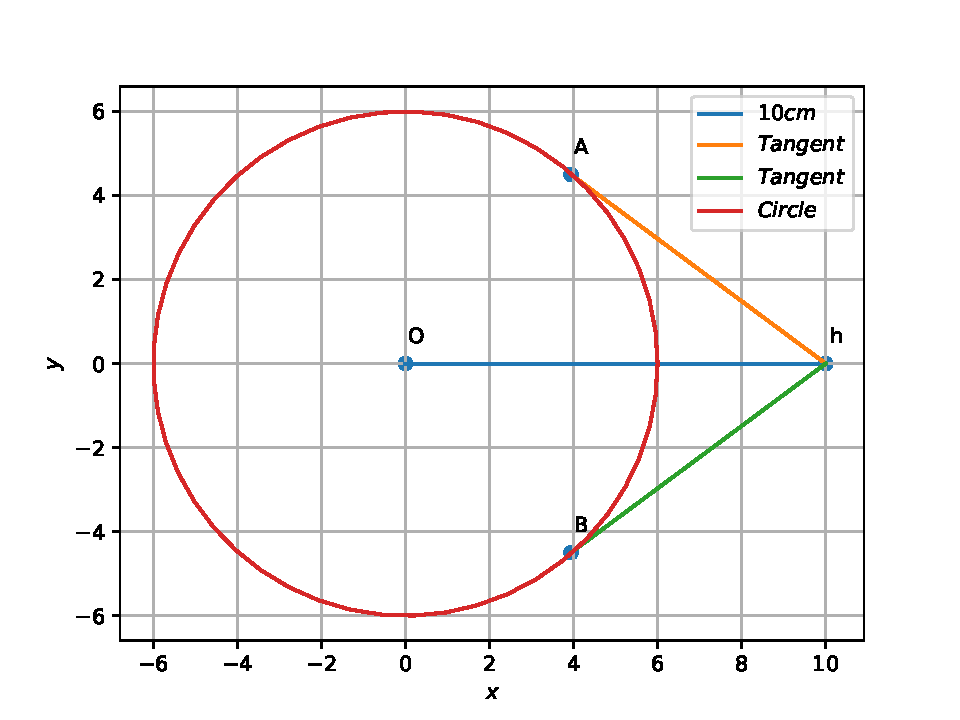
\includegraphics[width=\columnwidth]{chapters/10/11/2/1/figs/circle1.pdf}
		\caption{}
		\label{fig:10/11/2/1}
  	\end{figure}
	\\
	\solution  Follow the approach in Problem  
\ref{chapters/10/10/2/6}.
\iffalse
}

\section*{\large Solution}

\section*{\large Construction}

\begin{figure}[h]
\centering
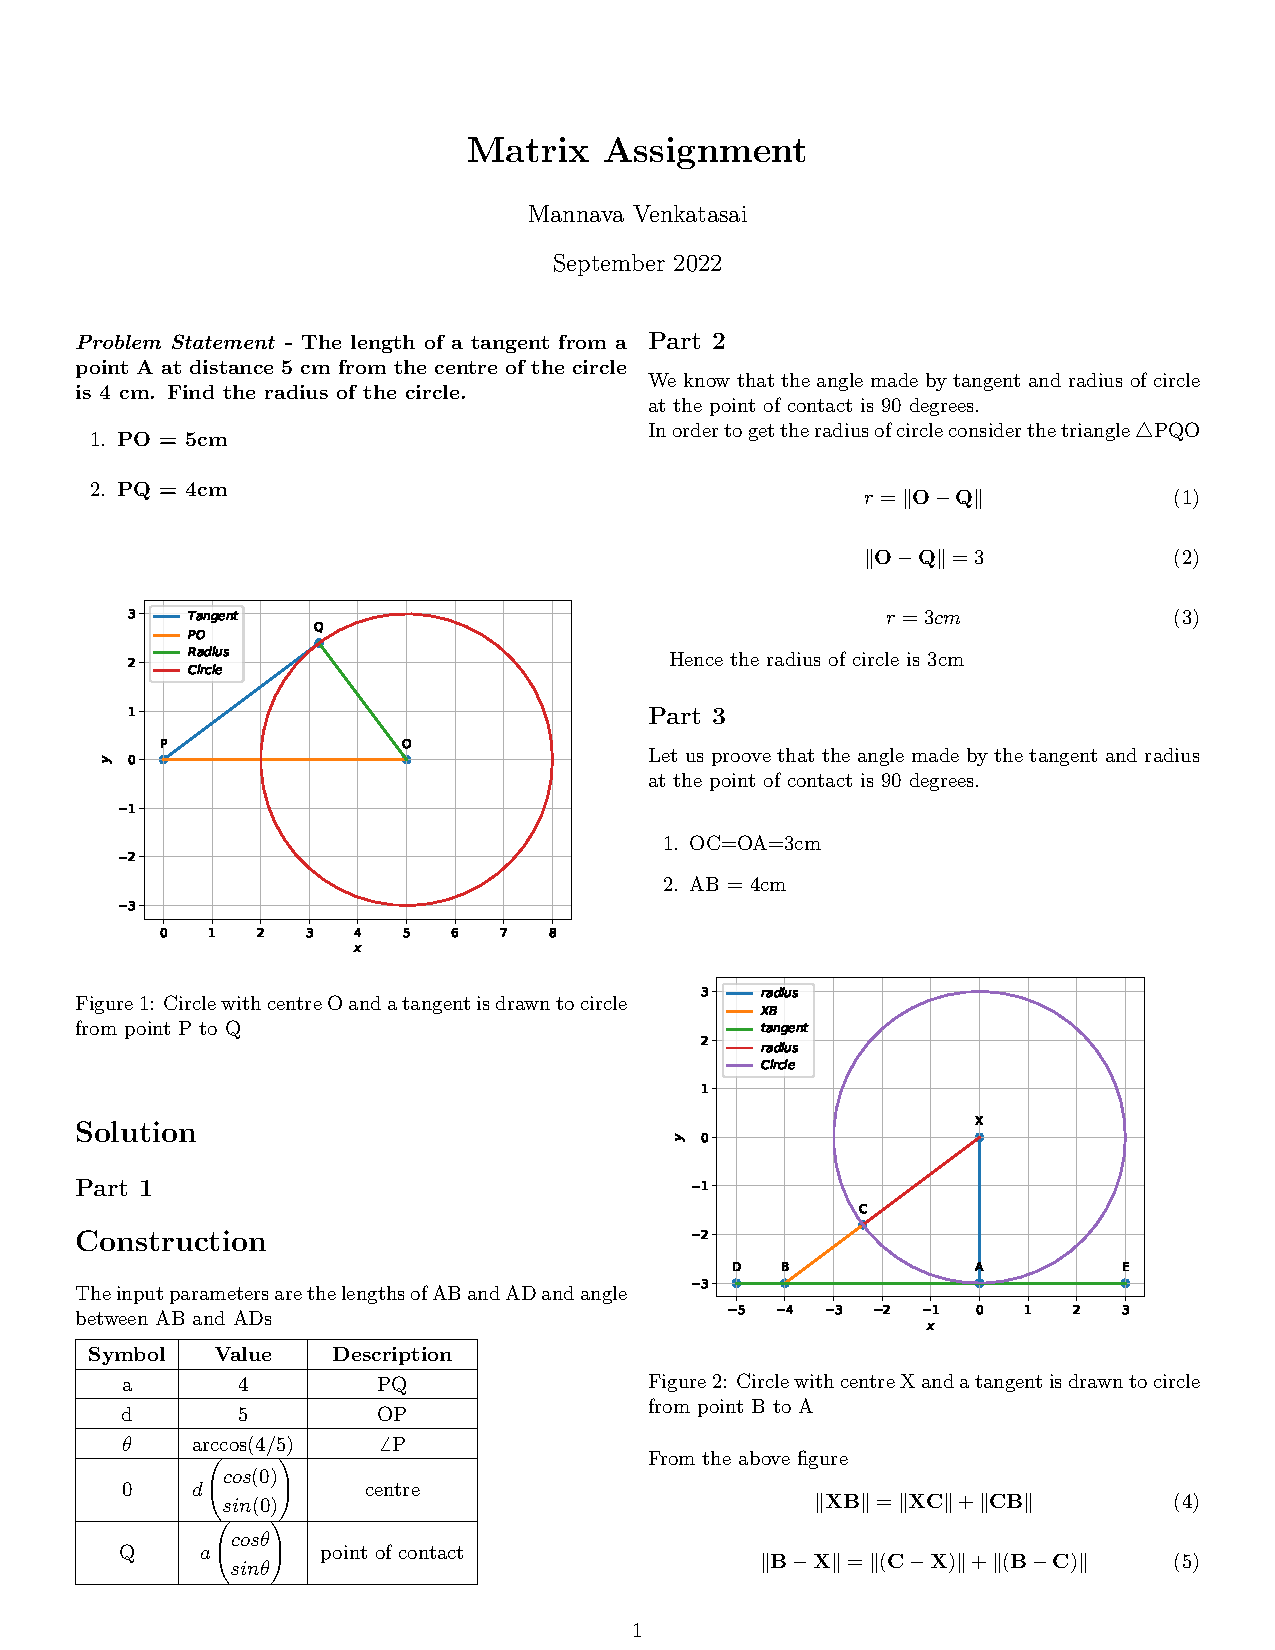
\includegraphics[width=1\columnwidth]{circle1.pdf}
\caption{Figure}
\label{fig:triangle}
\end{figure}

The dimensions of the figure is taken as below\\\\
{
\setlength\extrarowheight{2pt}
\centering
\begin{tabular}{|c|c|c|}
 \hline
 \textbf{Symbol}&\textbf{Value}&\textbf{Description}\\
 \hline
 r&6&Radius\\
 \hline
 h&10&distance\\
 \hline
 0&$d%
 \begin{pmatrix}
  cos(0)\\
  sin(0)\\
 \end{pmatrix}$%
 &centre\\
 \hline
 A&$a%
 \begin{pmatrix}
  cos\theta\\
  sin\theta\\
 \end{pmatrix}$%
 &point of contact\\
 \hline
 B&$b%
 \begin{pmatrix}
  cos\theta\\
  sin\theta\\
 \end{pmatrix}$%
 &point of contact\\
 \hline
\end{tabular}
}	
\\\\
	The equation of a conic with directrix $\vec{n^Tx}$ = c , eccentricity e anf focus $\boldsymbol{f}$ is given by
	
\begin{equation}
	\vec{x}^T\vec{V}\vec{x} + 2\vec{u}^T + f = 0
\end{equation}
	for circle eccentricity e = 0 then,\\
\begin{equation}
	\vec{V} = \vec{I} = \myvec{1&0\\0&1} , \vec{u} = \myvec{0\\0} , f = -r^2
\end{equation}
Point q on conic is given by 
\begin{equation}
	\vec{q} = \vec{V}^{-1}(\vec{n} - \vec{u})
\end{equation}
where, $\vec{n}$ is the normal vectors of the tangents from a point h to the conic are given by 
\begin{equation}
	\vec{n} = \frac{\vec{e_1}}{\vec{e_1^Th}} + \mu_i(\vec{Rh})
\end{equation}
\\
where $\mu _i$ 's are given by the following equation
\begin{equation}
	\mu_i = \frac{1}{\vec{{m^TVm}}}(\vec{-m^T(Vq+u)})	
\end{equation}
	 			$ \pm \sqrt{\vec{m^T(Vq+u)}^2 - (\vec{q^TVq + 2u^T} + f)(\vec{m^TVm)})}$
\\\\
$\mu _i$ 's are obtained by substituting the following in equation 6\\\\
\begin{equation}
	\vec{m} = (\vec{Rh})  ;  \vec{u}  = \myvec{0\\0}  ;  \vec{q} = \frac{\vec{e_1}}{\vec{e_1^Th}}
\end{equation}
 $\vec{R}$ = $\myvec{0&-1\\1&0}$ 
The obtained $\mu_i$'s are substituted in equation 5 and equation 5 is substituted in equation 6 the required points on conic A and B are obtained.\\\\
Now the point A and B are formed and tangents are drawn \\\\
To find the length of point h and point A \\
\begin{center}
	The distance between h and A is $\norm{\vec{h}-\vec{A}}$\\
\end{center}
\begin{equation}
  (\vec{h}-\vec{A})(\vec{h}-\vec{A})^T=d^2
\end{equation}
\begin{center}
	By solving  equation(7) we get \\
	    distance  d=$8cm$\\
	    \begin{equation}
  (\vec{h}-\vec{A})(\vec{h}-\vec{A})^T=d^2
\end{equation}
\end{center}
\begin{center}
	By solving  equation(7) we get \\
	    distance  d=$8cm$\\
	    \begin{equation}
	    \norm{\vec{h}-\vec{A}}=8cm
	    \end{equation}=8cm
\end{center}
To find the length of point h and point B\\
\begin{center}
	The distance between h and B is $\norm{\vec{h}-\vec{B}}$\\
\end{center}
\begin{equation}
  (\vec{h}-\vec{B})(\vec{h}-\vec{B})^T=d^2
\end{equation}
\begin{center}
	By solving  equation(10) we get \\
	    distance  d=$8cm$\\
	    \begin{equation}
	    \norm{\vec{h}-\vec{B}}=8cm
	    \end{equation}
	    from equation (9) and (11)\\
	    \begin{equation}
	    \norm{\vec{h}-\vec{A}}=\norm{\vec{h}-\vec{B}}
	    \end{equation}
	    \end{center}
	    Hence,the above equation (12) we can prove that the lenght of the tangents to a circle of radius 6cm,from a point 10cm away from the centre of the circle,is 8cm.\\
	    
	    
The below python code realizes the above construction:	\\
\begin{lstlisting}
https://github.com/soundaryanaru/FWC-assignments/blob/main/Matrix/circle_assignment/code/circle.py
\end{lstlisting}
\bibliographystyle{ieeetr}
\end{document}
\fi

\item 
\label{chapters/10/11/2/1}
\iffalse
\documentclass[journal,10pt,twocolumn]{article}
\usepackage{graphicx}
\usepackage[margin=0.5in]{geometry}
\usepackage[cmex10]{amsmath}
\usepackage{array}
\usepackage{booktabs}
\title{\textbf{Circle Assignment}}
\author{Soundarya Naru}
\date{October 2022}

\providecommand{\norm}[1]{\left\lVert#1\right\rVert}
\providecommand{\abs}[1]{\left\vert#1\right\vert}
\let\vec\mathbf
\newcommand{\myvec}[1]{\ensuremath{\begin{pmatrix}#1\end{pmatrix}}}
\newcommand{\mydet}[1]{\ensuremath{\begin{vmatrix}#1\end{vmatrix}}}
\providecommand{\brak}[1]{\ensuremath{\left(#1\right)}}
\usepackage{amsmath}
\usepackage{amssymb}
\usepackage{physics}
\usepackage{listings}
\usepackage{tabularx}

\begin{document}

\maketitle
\paragraph{\textit{Problem Statement:} \\
\fi
Draw a circle of radius 6 cm.
From a point 10 cm away from its centre, construct the pair of tangents to the circle and measure their lengths.
	\begin{figure}[!ht]
		\centering
 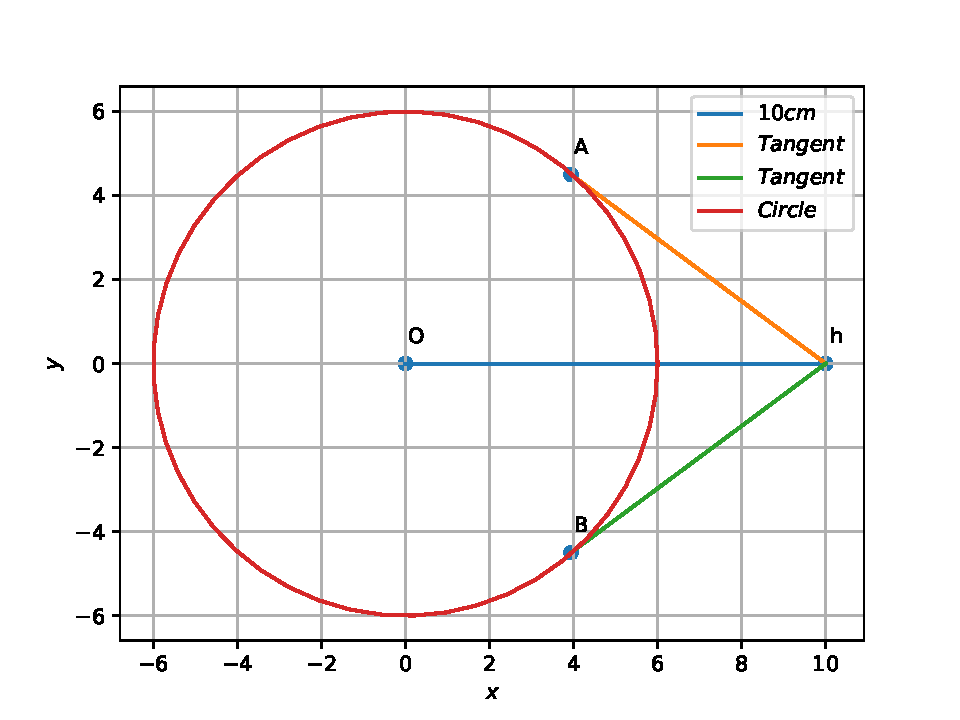
\includegraphics[width=\columnwidth]{chapters/10/11/2/1/figs/circle1.pdf}
		\caption{}
		\label{fig:10/11/2/1}
  	\end{figure}
	\\
	\solution  Follow the approach in Problem  
\ref{chapters/10/10/2/6}.
\iffalse
}

\section*{\large Solution}

\section*{\large Construction}

\begin{figure}[h]
\centering
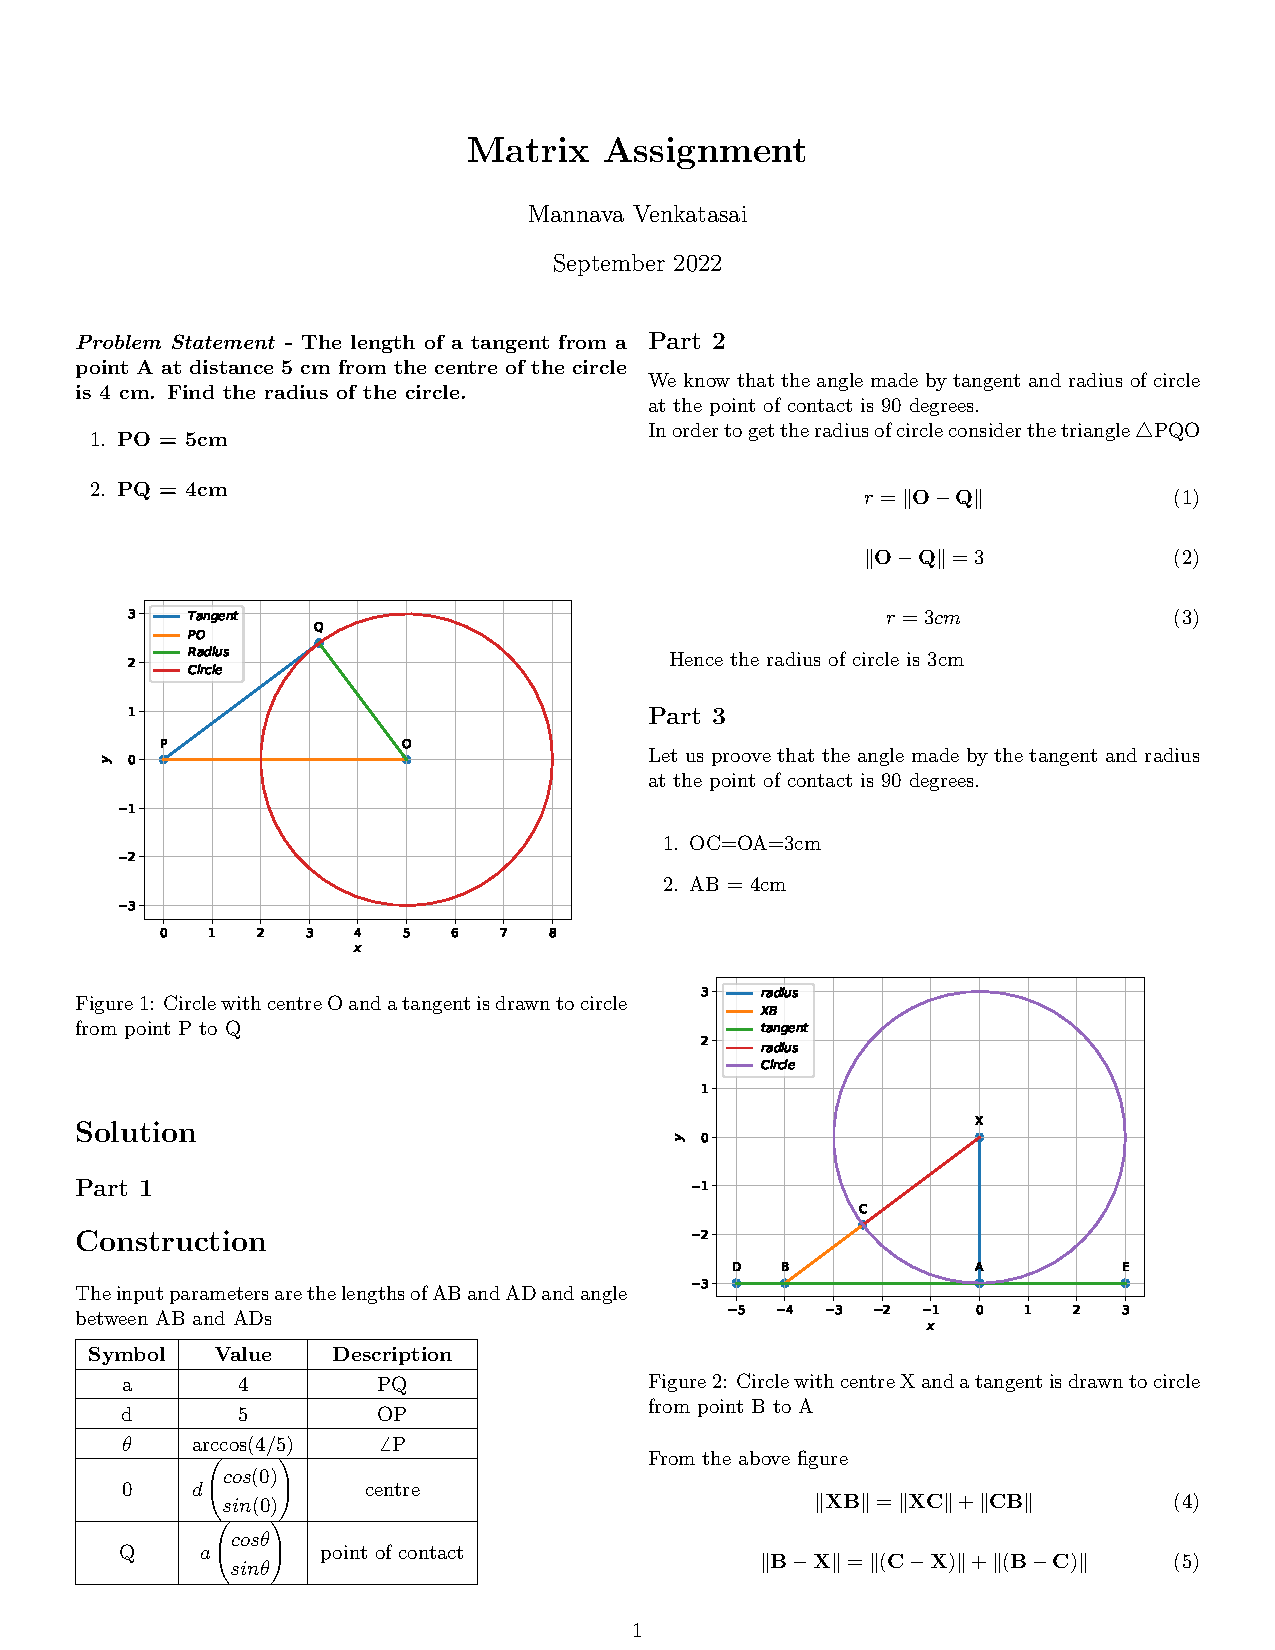
\includegraphics[width=1\columnwidth]{circle1.pdf}
\caption{Figure}
\label{fig:triangle}
\end{figure}

The dimensions of the figure is taken as below\\\\
{
\setlength\extrarowheight{2pt}
\centering
\begin{tabular}{|c|c|c|}
 \hline
 \textbf{Symbol}&\textbf{Value}&\textbf{Description}\\
 \hline
 r&6&Radius\\
 \hline
 h&10&distance\\
 \hline
 0&$d%
 \begin{pmatrix}
  cos(0)\\
  sin(0)\\
 \end{pmatrix}$%
 &centre\\
 \hline
 A&$a%
 \begin{pmatrix}
  cos\theta\\
  sin\theta\\
 \end{pmatrix}$%
 &point of contact\\
 \hline
 B&$b%
 \begin{pmatrix}
  cos\theta\\
  sin\theta\\
 \end{pmatrix}$%
 &point of contact\\
 \hline
\end{tabular}
}	
\\\\
	The equation of a conic with directrix $\vec{n^Tx}$ = c , eccentricity e anf focus $\boldsymbol{f}$ is given by
	
\begin{equation}
	\vec{x}^T\vec{V}\vec{x} + 2\vec{u}^T + f = 0
\end{equation}
	for circle eccentricity e = 0 then,\\
\begin{equation}
	\vec{V} = \vec{I} = \myvec{1&0\\0&1} , \vec{u} = \myvec{0\\0} , f = -r^2
\end{equation}
Point q on conic is given by 
\begin{equation}
	\vec{q} = \vec{V}^{-1}(\vec{n} - \vec{u})
\end{equation}
where, $\vec{n}$ is the normal vectors of the tangents from a point h to the conic are given by 
\begin{equation}
	\vec{n} = \frac{\vec{e_1}}{\vec{e_1^Th}} + \mu_i(\vec{Rh})
\end{equation}
\\
where $\mu _i$ 's are given by the following equation
\begin{equation}
	\mu_i = \frac{1}{\vec{{m^TVm}}}(\vec{-m^T(Vq+u)})	
\end{equation}
	 			$ \pm \sqrt{\vec{m^T(Vq+u)}^2 - (\vec{q^TVq + 2u^T} + f)(\vec{m^TVm)})}$
\\\\
$\mu _i$ 's are obtained by substituting the following in equation 6\\\\
\begin{equation}
	\vec{m} = (\vec{Rh})  ;  \vec{u}  = \myvec{0\\0}  ;  \vec{q} = \frac{\vec{e_1}}{\vec{e_1^Th}}
\end{equation}
 $\vec{R}$ = $\myvec{0&-1\\1&0}$ 
The obtained $\mu_i$'s are substituted in equation 5 and equation 5 is substituted in equation 6 the required points on conic A and B are obtained.\\\\
Now the point A and B are formed and tangents are drawn \\\\
To find the length of point h and point A \\
\begin{center}
	The distance between h and A is $\norm{\vec{h}-\vec{A}}$\\
\end{center}
\begin{equation}
  (\vec{h}-\vec{A})(\vec{h}-\vec{A})^T=d^2
\end{equation}
\begin{center}
	By solving  equation(7) we get \\
	    distance  d=$8cm$\\
	    \begin{equation}
  (\vec{h}-\vec{A})(\vec{h}-\vec{A})^T=d^2
\end{equation}
\end{center}
\begin{center}
	By solving  equation(7) we get \\
	    distance  d=$8cm$\\
	    \begin{equation}
	    \norm{\vec{h}-\vec{A}}=8cm
	    \end{equation}=8cm
\end{center}
To find the length of point h and point B\\
\begin{center}
	The distance between h and B is $\norm{\vec{h}-\vec{B}}$\\
\end{center}
\begin{equation}
  (\vec{h}-\vec{B})(\vec{h}-\vec{B})^T=d^2
\end{equation}
\begin{center}
	By solving  equation(10) we get \\
	    distance  d=$8cm$\\
	    \begin{equation}
	    \norm{\vec{h}-\vec{B}}=8cm
	    \end{equation}
	    from equation (9) and (11)\\
	    \begin{equation}
	    \norm{\vec{h}-\vec{A}}=\norm{\vec{h}-\vec{B}}
	    \end{equation}
	    \end{center}
	    Hence,the above equation (12) we can prove that the lenght of the tangents to a circle of radius 6cm,from a point 10cm away from the centre of the circle,is 8cm.\\
	    
	    
The below python code realizes the above construction:	\\
\begin{lstlisting}
https://github.com/soundaryanaru/FWC-assignments/blob/main/Matrix/circle_assignment/code/circle.py
\end{lstlisting}
\bibliographystyle{ieeetr}
\end{document}
\fi

\fi
\item 
\item 
\item 
\item 
\item 
\item 
\item 
\item 
\item 
\label{chapters/11/10/2/9}
\iffalse
\documentclass[journal,12pt,twocolumn]{IEEEtran}
\usepackage{graphicx}
\usepackage[margin=0.5in]{geometry}
\graphicspath{{./figs/}}{}
\usepackage{amsmath,amssymb,amsfonts,amsthm}
\newcommand{\myvec}[1]{\ensuremath{\begin{pmatrix}#1\end{pmatrix}}}
\usepackage{listings}
\usepackage{watermark}
\usepackage{titlesec}
\let\vec\mathbf
\lstset{
frame=single, 
breaklines=true,
columns=fullflexible
}
%\thiswatermark{\centering \put(0,-105.0){
\includegraphics[scale=0.5]{iith.png}} }

\title{\mytitle}
\title{
Matrix Assignment - Lines
}
\author{Adarsh Kumar (FWC22068)}
\begin{document}
\maketitle
\tableofcontents
\bigskip


\section{\textbf{Problem}}
\fi
The Vertices of Triangle $PQR$ is $\vec{P}(2,1), \vec{Q}(-2,3), \vec{R}(4,5)$. Find the equation of the Median Through $\vec{R}$.
	\begin{figure}[!ht]
		\centering
 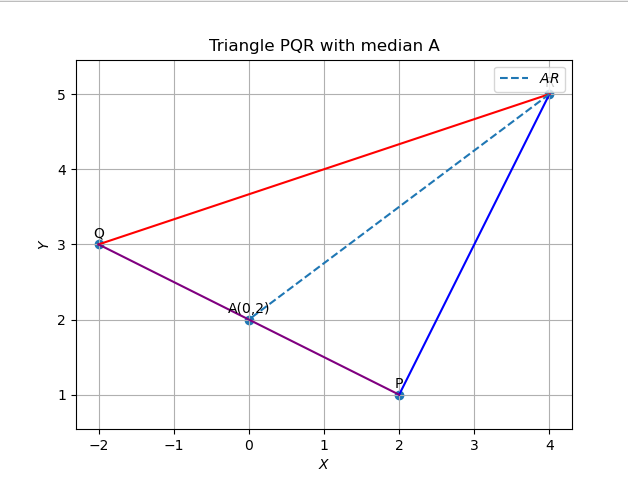
\includegraphics[width=\columnwidth]{chapters/11/10/2/9/figs/line.png}
		\caption{}
		\label{fig:11/10/2/9}
  	\end{figure}
	\\
	\solution See Fig. 
		\ref{fig:11/10/2/9}.
\iffalse


\section{\textbf{Solution}}
Given the Vertices are :\\
\linebreak
$\vec{P} = \myvec{2 \\ 1}$ \hspace{5mm}
$\vec{Q} = \myvec{-2 \\ 3}$ \hspace{5mm}
$\vec{R} = \myvec{4 \\ 5}$ \hspace{5mm}
\linebreak


We know that the Median through R ,
will divide the side PQ in two equal parts.
\\
We know that the the median through R will
divide or intersect the side PQ into two equal parts.
\\
So , By using section formula , we can find the Coordinates of the point A(say) on PQ where the median intersect the side PQ.

\textbf{Section Formula :}

\begin{align}
 Point A = \frac{P + K(Q)}{1+K}  \label{eq-1}
\end{align}
\\
where PQ is a line and P and Q is the coordinates and K is the ratio in which the line is being divided.
\\

Now , we know that the Median from R will divide the side PQ in two equal parts 
\\( i.e in th ratio 1 : 1 )

So ,  by 
\fi
Using Section Formula,
\begin{align}
\vec{A} &= \frac{\vec{P} +\vec{Q} }{2}
\\
	&= {\myvec{0\\2}}
\end{align} 
\iffalse
Now ,our Aim is to find the equation of Median(line AR)

So, Now we have two points \\
\linebreak
$\vec{A} = \myvec{0 \\ 2}$ \hspace{5mm}
$\vec{R} = \myvec{4 \\ 5}$ \\
\linebreak
We know that ,\\
The Parametric Equation of line is :\\
\begin{align}
\vec{X} = \vec{A}+\lambda\vec{m}
\end{align}
Where \textbf{m} is the direction vector of the line\\
\linebreak
\fi
So , the Direction Vector of $AR$ is 
\begin{align}
	\vec{m} &={\vec{R} - \vec{A}}
= \myvec{4 \\ 3}
\\
	\implies \vec{n} &= 
 \myvec{3 \\ -4}
\end{align}
which is the normal vector.  Thus, from
    \eqref{eq:line_norm_eq},
the equation of the line is 
\begin{align}
	\myvec{3 & -4}\brak{\vec{x} - \vec{R}} = 0
	\\
	\implies 
	\myvec{3 & -4}\vec{x} =8 
\end{align}
\iffalse
Therefore the equation of line AR will be:
\begin{align}
\vec{X} = \myvec{0 \\ 2}+\lambda\myvec{ 4 \\ 3}
\end{align}
Equation 9 ,represents the equation of line AR in Parametric Form . 

\newpage


\section{\textbf{Figure}}
\begin{figure}[h]
    \centering
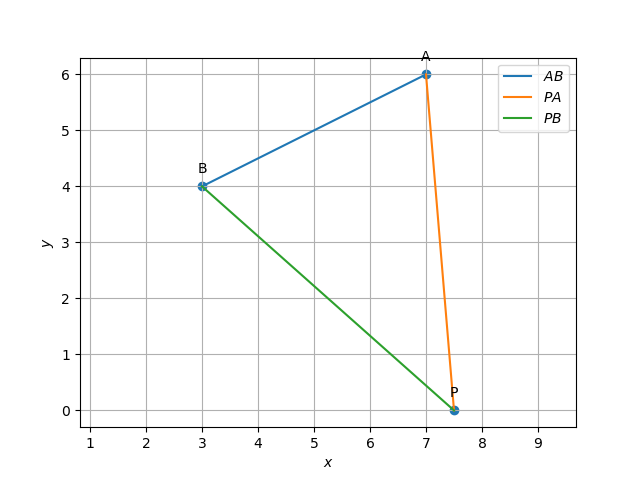
\includegraphics[width=\columnwidth]{line.png}
    \label{fig:my_label}
\end{figure}


\section*{Construction}
The dimensions of the Triangle made by using Python  are taken as below\\
\linebreak
{
\centering
	\begin{tabular}{|c|c|}
	\hline
	\textbf{vertex}&\textbf{co-ordinates}\\
	\hline
	P&(2,1)\\
	\hline
	Q&(-2,3)\\
	\hline
	R&(4,5)\\
	\hline
	A&(0,2)\\
	\hline
\end{tabular}
}
\section{\textbf{Code Link}}

\begin{lstlisting}
https://github.com/aadrshptel/Fwc_module1/tree/main/Assignments/Matrix%20assignments/Lines/codes
\end{lstlisting}
Execute the code by using the command\\
\textbf{python3 line.py}



\end{document}
\fi

\item 
\label{chapters/11/10/2/10}
\def\mytitle{LINE USING PYTHON}
\def\myauthor{Mukesh Guptha.CH}
\def\contact{mukeshchinta1313@gmail.com}
\def\mymodule{Future Wireless Communication (FWC)}
\documentclass[10pt, a4paper]{article}
\usepackage[a4paper,outer=1.5cm,inner=1.5cm,top=1.75cm,bottom=1.5cm]{geometry}
\twocolumn
\usepackage{graphicx}
\graphicspath{{./images/}}
\usepackage[colorlinks,linkcolor={black},citecolor={blue!80!black},urlcolor={blue!80!black}]{hyperref}
\usepackage[parfill]{parskip}
\usepackage{lmodern}
\usepackage{tikz}
	\usepackage{physics}
%\documentclass[tikz, border=2mm]{standalone}
\usepackage{karnaugh-map}
%\documentclass{article}
\usepackage{tabularx}
\usepackage{circuitikz}
\usetikzlibrary{calc}
\usepackage{amsmath}
\usepackage{amssymb}
\renewcommand*\familydefault{\sfdefault}
\usepackage{watermark}
\usepackage{lipsum}
\usepackage{xcolor}
\usepackage{listings}
\usepackage{float}
\usepackage{titlesec}
\providecommand{\mtx}[1]{\mathbf{#1}}
\titlespacing{\subsection}{1pt}{\parskip}{3pt}
\titlespacing{\subsubsection}{0pt}{\parskip}{-\parskip}
\titlespacing{\paragraph}{0pt}{\parskip}{\parskip}
\newcommand{\figuremacro}[5]{
    \begin{figure}[#1]
        \centering
        \includegraphics[width=#5\columnwidth]{#2}
        \caption[#3]{\textbf{#3}#4}
        \label{fig:#2}
    \end{figure}
}
\newcommand{\myvec}[1]{\ensuremath{\begin{pmatrix}#1\end{pmatrix}}}
\let\vec\mathbf
\lstset{
frame=single, 
breaklines=true,
columns=fullflexible
}

\title{\mytitle}
\author{\myauthor\hspace{1em}\\\contact\\FWC22069\hspace{6.5em}IITH\hspace{0.5em}\mymodule\hspace{6em}ASSIGN-4}
\date{}
\begin{document}
	\maketitle
 \paragraph*{\large Problem Statement}
$-$ \textbf{ Find the equation of the line passing through  (-3,5) and perpendicular to the line through the points (2,5) and (-3,6).}
 
\begin{figure}[h]
\centering
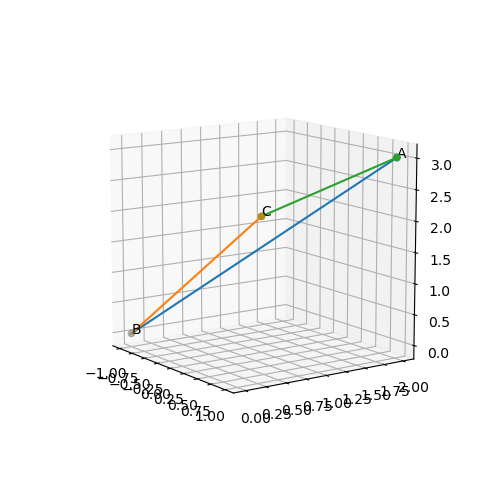
\includegraphics[width=1\columnwidth]{Figure_1.png}
\caption{perpendicular intersection}
\end{figure}
	\section*{Construction}
\vspace{2mm}
 the input parameters are as follows
{
\setlength\extrarowheight{4pt}
 
 \begin{tabular}{|c|c|c|}
	\hline
	\textbf{Symbol}&\textbf{Value}&\textbf{Description}\\
	\hline
 c&$
	\begin{pmatrix}
		5\\
		-1\\
	\end{pmatrix}$
	&coefficients of line \\
	\hline
 d&$
	\begin{pmatrix}
		20\\
	\end{pmatrix}$
	&constants\\
	\hline
 \end{tabular}
}
\section*{\large solution}

\subsection*{\large part 1}
let us take A=(2,5),B=(-3,6) and P=(-3,5).Directional vector  of the points\vspace{4mm}m=B-A\\
\begin{equation}
m=\begin{pmatrix}
    2\\
    5\\
\end{pmatrix}-\begin{pmatrix}
    -3\\
    6\\
\end{pmatrix}\hspace{2em}
m=\begin{pmatrix}
    5\\
    -1\\
\end{pmatrix}
\label{eq-1}
\end{equation}


\begin{eqnarray}
\vec{m^t\vec{(X-P)}}=0
\end{eqnarray}
\begin{equation}
\begin{pmatrix}
    5 &-1\\
\end{pmatrix}\begin{pmatrix}
    X-P\\
\end{pmatrix}
    \label{eq-3}
\end{equation}

\begin{equation}
 \begin{pmatrix}
    5 & -1\\
\end{pmatrix}\begin{pmatrix}
    x+3\\
    y-5\\
\end{pmatrix}
\label{eq-4}
\end{equation}
The required line equation is 
\begin{equation}
 5\vec{x}-\vec{y}+20=0
\label{eq-5}
\end{equation}
\end{document}
\item 
\label{chapters/11/10/2/11}
\documentclass[journal,12pt,twocolumn]{article}
\usepackage{graphicx}
\graphicspath{{./figs/}}{}
\usepackage{amsmath,amssymb,amsfonts,amsthm}
\newcommand{\myvec}[1]{\ensuremath{\begin{pmatrix}#1\end{pmatrix}}}
\let\vec\mathbf
\title{
Matrix-Lines
}
\author{SHREYASH CHANDRA PUTTA}
\begin{document}
\maketitle
\tableofcontents

\section{Problem Statement}
A line perpendicular to the line segement joining the points (1,0)and(2,3)divides it in the ratio 1:n . find the equation of the line?\\
(note: we are taking n as user Input) .

% 

\begin{table}[h]
    \centering
    \begin{tabular}{|c|c|c|}
       \hline
       \textbf{Symbol}&\textbf{Value}&\textbf{Description}  \\
       \hline
	    $\vec{P}$ & $\myvec{
		    1\\
		    0}$
	    & given point\\
        \hline
	    $\vec{Q}$ & $\myvec{2\\3}$
 & given point\\
        \hline
	    $\vec{R}$ & $\myvec{
  \frac{2+n}{1+n}\\
  \frac{3}{1+n}}$
 & intersecting point  \\
       \hline
    \end{tabular}
    \caption{Parameters}
    \label{tab:my_label}
\end{table}

%\section{Construction}

\begin{figure}[h]
    \centering
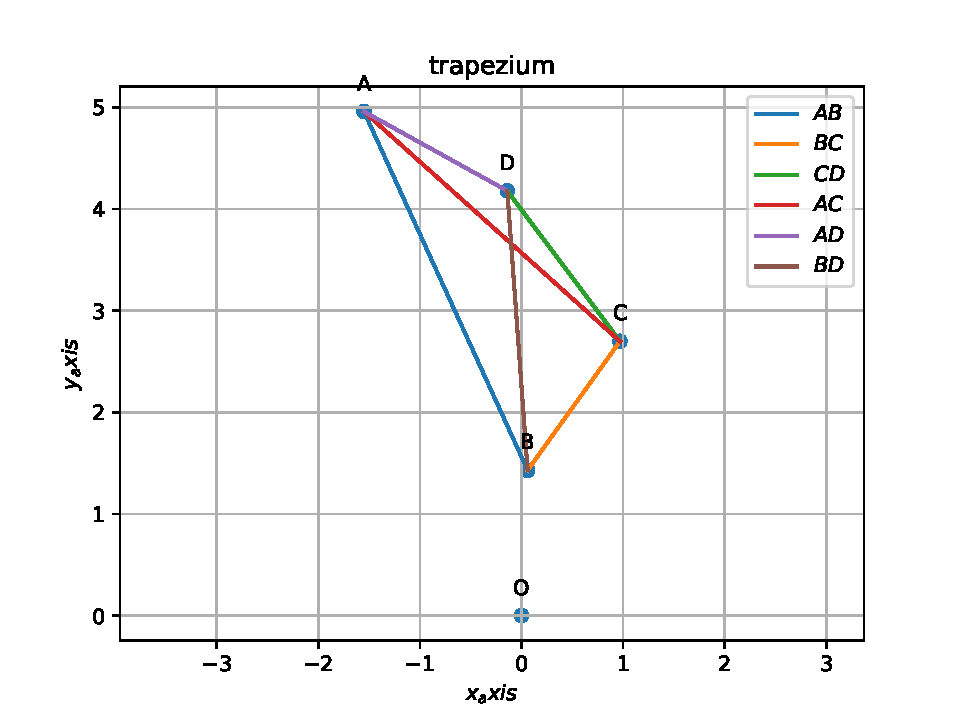
\includegraphics[width=\columnwidth]{fig/linefig.pdf}
    \caption{Equation of the required Straight Line}
    \label{fig:my_label}
\end{figure}




\section{Solution}

Given that resultant will divide the equation of line in the ratio 1:n and the line is perpendicular to line segment joining the points (1,0)and(2,3)  ) \\
%so, b = 9 - a  \\
\\
Let ${\vec{P}}$=$\myvec{
  1\\
  0}$
 and ${\vec{Q}}$=$\myvec{
  2\\
  3}$
\\
\\
Equation of line is ${\vec{n^{\top}}\vec{X}} = c$.
\\
\\
We know if 2 points of the linesegment is given then,\\
 %The Equation of line through ${\vec{P}}$ is\\
%\begin{equation}
%	\vec{n^{\top}}
%	\myvec{
 % a\\
  %0}
  %= c \label{eq-1}
%\end{equation}
\\
Direction vector of line joining two points  ${\vec{P}}$ ${\vec{Q}}$ is given by\\

\begin{equation}
	\vec{M}=
     \vec{Q
 }-  \vec{P
 }
  \label{eq-2}
\end{equation}
\\

\begin{equation}
	\vec{M}=
     \myvec{
  2\\
  3
 }-  \myvec{
  1\\
  0
 }
  \label{eq-2}
\end{equation}
\\
\\
\begin{equation}
	\vec{M}=
     \myvec{
  1\\
  3
 }
   \label{eq-2}
\end{equation}
\\
We know, that position or  directional vector of points P and Q line segement used as the normal vector
\\
\\
 The general equation of the required perpendicular line is
 ${\vec{M^{\top}}\vec{X}} = c$.
 \\
 \\
 The perpendicular line cutting a line segment P and Q in ratio 1:n is passes through the point R.
 
 \begin{equation}
	 \vec{R}=\frac{\vec{Q}+n\vec{P}}{1+n}
	 \label{eq-4}
\end{equation}
 \\
Equation of line passing through ${\vec{R}}$ is\\
\begin{equation}
	\vec{M^{\top}}(\vec{X}-\vec{R})=0
	 \label{eq-4}
\end{equation}
\\
\begin{equation}
	 \vec{M^{\top}}
	 \vec{X} - \vec{M^{\top}}
	 \vec{R} = 0
	 \label{eq-5}
\end{equation}
 \\
 From eq4, eq6 and eq3 we can find the required Perpenducular line equation. 
 \begin{equation}
	   \myvec{
  1\  3}\vec{X}
	 = \myvec{
  1\ 3}\myvec{
  \frac{2+n}{1+n}\\
  \frac{3}{1+n}} 
  \label{eq-5}
\end{equation}
\\
Therefore the equation of a line perpendicular to the given line segement divides it in the ratio 1:n is:
 \begin{equation}
	   \myvec{
  1\  3}\vec{X}
	 = \frac{11+n}{1+n} 
  \label{eq-5}
\end{equation}



 
\section{Software}
Download the following code using,
\begin{table}[h]
    \centering
    \begin{tabular}{|c|}
    \hline \\
         svn co https://github.com/chanduputta/ \\FWC-Module1Assignments/blob/\\main/assignment4/line/lines3.py  \\
         \\
\hline
    \end{tabular}
\end{table}
\\
and execute the code by using command
\begin{center}
	\textbf{cmd:}
{Python3  lines3.py}\\
	\textbf{Then,}
{input your required n value}
\end{center}

\section{Conclusion}
\begin{center}
We found the equation of a line perpendicular to the line segement joining the points (1,0)and(2,3) divides it in the ratio 1:n .
\end{center}
\end{document}

\item 
%\label{chapters/11/10/2/11}
%\documentclass[journal,12pt,twocolumn]{article}
\usepackage{graphicx}
\graphicspath{{./figs/}}{}
\usepackage{amsmath,amssymb,amsfonts,amsthm}
\newcommand{\myvec}[1]{\ensuremath{\begin{pmatrix}#1\end{pmatrix}}}
\let\vec\mathbf
\title{
Matrix-Lines
}
\author{SHREYASH CHANDRA PUTTA}
\begin{document}
\maketitle
\tableofcontents

\section{Problem Statement}
A line perpendicular to the line segement joining the points (1,0)and(2,3)divides it in the ratio 1:n . find the equation of the line?\\
(note: we are taking n as user Input) .

% 

\begin{table}[h]
    \centering
    \begin{tabular}{|c|c|c|}
       \hline
       \textbf{Symbol}&\textbf{Value}&\textbf{Description}  \\
       \hline
	    $\vec{P}$ & $\myvec{
		    1\\
		    0}$
	    & given point\\
        \hline
	    $\vec{Q}$ & $\myvec{2\\3}$
 & given point\\
        \hline
	    $\vec{R}$ & $\myvec{
  \frac{2+n}{1+n}\\
  \frac{3}{1+n}}$
 & intersecting point  \\
       \hline
    \end{tabular}
    \caption{Parameters}
    \label{tab:my_label}
\end{table}

%\section{Construction}

\begin{figure}[h]
    \centering
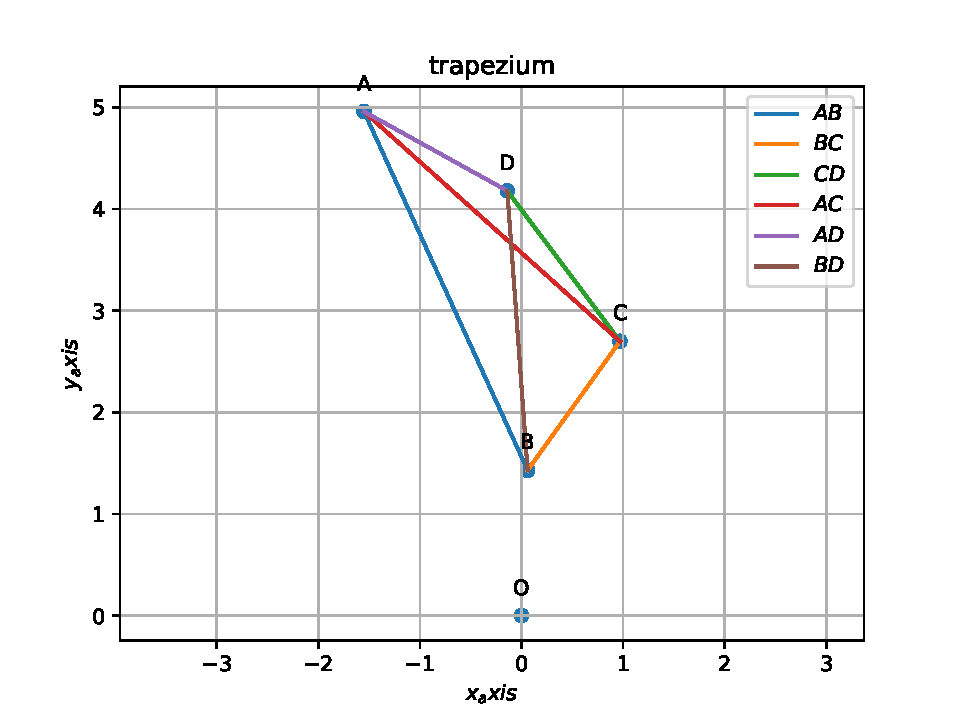
\includegraphics[width=\columnwidth]{fig/linefig.pdf}
    \caption{Equation of the required Straight Line}
    \label{fig:my_label}
\end{figure}




\section{Solution}

Given that resultant will divide the equation of line in the ratio 1:n and the line is perpendicular to line segment joining the points (1,0)and(2,3)  ) \\
%so, b = 9 - a  \\
\\
Let ${\vec{P}}$=$\myvec{
  1\\
  0}$
 and ${\vec{Q}}$=$\myvec{
  2\\
  3}$
\\
\\
Equation of line is ${\vec{n^{\top}}\vec{X}} = c$.
\\
\\
We know if 2 points of the linesegment is given then,\\
 %The Equation of line through ${\vec{P}}$ is\\
%\begin{equation}
%	\vec{n^{\top}}
%	\myvec{
 % a\\
  %0}
  %= c \label{eq-1}
%\end{equation}
\\
Direction vector of line joining two points  ${\vec{P}}$ ${\vec{Q}}$ is given by\\

\begin{equation}
	\vec{M}=
     \vec{Q
 }-  \vec{P
 }
  \label{eq-2}
\end{equation}
\\

\begin{equation}
	\vec{M}=
     \myvec{
  2\\
  3
 }-  \myvec{
  1\\
  0
 }
  \label{eq-2}
\end{equation}
\\
\\
\begin{equation}
	\vec{M}=
     \myvec{
  1\\
  3
 }
   \label{eq-2}
\end{equation}
\\
We know, that position or  directional vector of points P and Q line segement used as the normal vector
\\
\\
 The general equation of the required perpendicular line is
 ${\vec{M^{\top}}\vec{X}} = c$.
 \\
 \\
 The perpendicular line cutting a line segment P and Q in ratio 1:n is passes through the point R.
 
 \begin{equation}
	 \vec{R}=\frac{\vec{Q}+n\vec{P}}{1+n}
	 \label{eq-4}
\end{equation}
 \\
Equation of line passing through ${\vec{R}}$ is\\
\begin{equation}
	\vec{M^{\top}}(\vec{X}-\vec{R})=0
	 \label{eq-4}
\end{equation}
\\
\begin{equation}
	 \vec{M^{\top}}
	 \vec{X} - \vec{M^{\top}}
	 \vec{R} = 0
	 \label{eq-5}
\end{equation}
 \\
 From eq4, eq6 and eq3 we can find the required Perpenducular line equation. 
 \begin{equation}
	   \myvec{
  1\  3}\vec{X}
	 = \myvec{
  1\ 3}\myvec{
  \frac{2+n}{1+n}\\
  \frac{3}{1+n}} 
  \label{eq-5}
\end{equation}
\\
Therefore the equation of a line perpendicular to the given line segement divides it in the ratio 1:n is:
 \begin{equation}
	   \myvec{
  1\  3}\vec{X}
	 = \frac{11+n}{1+n} 
  \label{eq-5}
\end{equation}



 
\section{Software}
Download the following code using,
\begin{table}[h]
    \centering
    \begin{tabular}{|c|}
    \hline \\
         svn co https://github.com/chanduputta/ \\FWC-Module1Assignments/blob/\\main/assignment4/line/lines3.py  \\
         \\
\hline
    \end{tabular}
\end{table}
\\
and execute the code by using command
\begin{center}
	\textbf{cmd:}
{Python3  lines3.py}\\
	\textbf{Then,}
{input your required n value}
\end{center}

\section{Conclusion}
\begin{center}
We found the equation of a line perpendicular to the line segement joining the points (1,0)and(2,3) divides it in the ratio 1:n .
\end{center}
\end{document}

\item 
\label{chapters/11/10/2/13}
\iffalse
\documentclass[journal,12pt,twocolumn]{IEEEtran}
\usepackage{graphicx}
\graphicspath{{./figs/}}{}
\usepackage{amsmath,amssymb,amsfonts,amsthm}
\newcommand{\myvec}[1]{\ensuremath{\begin{pmatrix}#1\end{pmatrix}}}

\let\vec\mathbf

\title{
Matrix-Lines
}
\author{Kukunuri Sampath Govardhan}
\begin{document}
\maketitle
\tableofcontents
\bigskip
\section{Problem Statement}
\fi
Find equation of a line passing trough a point (2,2) and cutting off intercepts on the axes whose sum is 9.
	\begin{figure}[!ht]
		\centering
 \includegraphics[width=\columnwidth]{chapters/11/10/2/13/figs/assign4.png}
		\caption{}
		\label{fig:11/10/2/13}
  	\end{figure}
	\\
	\solution 
\iffalse
\section{Construction}
\begin{figure}[h]
    \centering
\includegraphics[width=\columnwidth]{figs/assign4.png}
    \caption{Equation of the Straight Line}
    \label{fig:my_label}
\end{figure}
\vspace{2cm}
\begin{table}[h]
    \centering
    \begin{tabular}{|c|c|c|}
       \hline
       \textbf{Symbol}&\textbf{Value}&\textbf{Description}  \\
       \hline
	    $\vec{P}$ & $\myvec{
		    a\\
		    0}$
	    & Point on X-axis\\
        \hline
	    $\vec{Q}$ & $\myvec{0\\b}$
 & Point on Y-axis\\
        \hline
	    $\vec{R}$ & $\myvec{
  2\\
  2}$
 & Given Point \\
        \hline
        a + b & 9 & Given Condition\\
        \hline
    \end{tabular}
    \caption{Parameters}
    \label{tab:my_label}
\end{table}


\section{Solution}
Given that resultant line passes through point(2,2) and intercepts on axes whose sum is 9 (
\fi
Let the $x$ intercept be $a$ and the $y$ intercept be $b$. 
Then 
\begin{align}
		\label{eq:11/10/2/13-a+b}
 a + b = 9
\end{align}
Let 
\begin{align}
{\vec{P}}=\myvec{
  a\\
  0}
 , {\vec{Q}}=\myvec{
  0\\
  b}
  , {\vec{R}}=\myvec{
  2\\
  2}
\end{align}
Since the points are collinear, from 
	\eqref{eq:normal_line-collinear},
	we obtain the matrix
\begin{align}
	\myvec{ \vec{P}-\vec{Q} &\vec{P}-\vec{R}} 
	=
	 \myvec{
  a & a-2\\
  -b & -2
 }
\end{align}
which is singular if the determinant
\begin{align}
	-2a +b(a-2) = ab -2\brak{a+b} = 0
\end{align}
yielding
\begin{align}
	ab = 18
		\label{eq:11/10/2/13-ab}
\end{align}
upon substituting from 
		\eqref{eq:11/10/2/13-a+b}.
		\eqref{eq:11/10/2/13-ab}
		and 
		\eqref{eq:11/10/2/13-a+b}
		form
\begin{align}
	x^2 -9x +18 = 0
\end{align}
with roots
\begin{align}
	x = 6,3
	\\
	\text{or, }
	\myvec{a \\ b} = \myvec{6 \\ 3}, \myvec{3\\6}
\end{align}
Since the direction vector of the line is 
\begin{align}
	\vec{P}-\vec{Q} = \myvec{a \\ -b},
\end{align}
the normal vector is 
\begin{align}
	\vec{n} = \myvec{b \\ a} \equiv \myvec{1 \\ 2}, \myvec{2\\1}
\end{align}
Thus, the possible equations of the line are 
\begin{align}
\myvec{1 & 2}\vec{x} = 6
	\\
	\myvec{2&1}\vec{x} = 6
\end{align}
\iffalse
\\
\\
Equation of line is ${\vec{n^{\top}}\vec{X}} = c$.\\
\\
Now we have 3 points which lies on same line so,\\
 The Equation of line through ${\vec{P}}$ is\\
 Hence, 
\begin{align}
	\vec{n}^{\top}
	\myvec{
  a\\
  0}
  &= c 
\\
	\vec{n}^{\top}
     \myvec{
  0\\
  b
 }
	&= c 
  \\
  \implies 
	\vec{n}^{\top}
	\myvec{
  a\\
  b
}
	&= 2c 
\end{align}
upon addition.
Also, 
\begin{align}
	\vec{n}^{\top}
	\myvec{
  2\\
  2}
  = c 
\end{align}
	Thus, we obtain, upon clubbing the above two equations,
 \begin{align}
	 \vec{n}^{\top}
	 \myvec{
  a & 9-a\\
  2 & 2
 }
	 = c\myvec{
  2\\
  1}
\end{align}
yielding
 \begin{align}
	 \vec{n^{\top}} &= 
	 \myvec{
  a & 9-a\\
  2 & 2
 }
  ^{-1}
	 \myvec{
  2\\
  1}
 c 
\end{align}
%
  \\
  Thus, we get \textbf{a = 2, b = 9-a = 7}\\
  \\
  by substuting a in eq6, finally\\
  \\
   \begin{align}
	   \vec{n^{\top}} = 
	   \myvec{
  0.3\\
  0.2}
 .c
 \end{align}
  \\
The Resultant Equation of line is ${\vec{n^{\top}}\vec{X}} = c$ \\
\\
 \begin{align}
	 \myvec{
  0.3\\
  0.2\\
 }
	 .\vec{X}.c = c
 \end{align}
  \\
i.e,    \\
\begin{align}
	\myvec{
  3\\
  2}
	.\vec{X} = 10
 \end{align}
\\
\textbf{
Therefore equation of the line is, \\
\begin{align}
	\myvec{
  3\\
  2}
	. \vec{X} = 10
 \end{align}}
\begin{center}
    \textbf{3x + 2y = 10}
\end{center}
\section{Software}
Download the following code using,
\begin{table}[h]
    \centering
    \begin{tabular}{|c|}
    \hline \\
         svn co https://github.com/\\mygit-sampath-govardhan/fwc-iith-assignments/blob/\\5b65abbf8e5e3c803b1bff8cf4a95092e100de75/\\Assignment-4(Matrices-line)/codes/Assignment4.py  \\
         \\
\hline
    \end{tabular}
\end{table}
\\
and execute the code by using command
\begin{center}
\textbf{Python3  Assignment4.py}\\
\end{center}

\section{Conclusion}
We found the equation of a line passing trough a point
(2,2) and cutting off intercepts on the axes whose
sum is 9.

\end{document}
\fi

\item 
\label{chapters/11/10/2/14}
\iffalse
\documentclass[journal,10pt,twocolumn]{article}
\usepackage{graphicx, float}
\usepackage[margin=0.5in]{geometry}
\usepackage{amsmath, bm}
\usepackage{array}
\usepackage{booktabs}
\usepackage{xfrac}

\providecommand{\norm}[1]{\left\lVert#1\right\rVert}
\let\vec\mathbf
\newcommand{\myvec}[1]{\ensuremath{\begin{pmatrix}#1\end{pmatrix}}}
\newcommand{\mydet}[1]{\ensuremath{\begin{vmatrix}#1\end{vmatrix}}}

\title{\textbf{Line Assignment}}
\author{Harsha sai sampath kumar}
\date{September 2022}

\begin{document}

\maketitle
\paragraph{\textit{\large Problem Statement} -
\fi
Find the equation of the line through the point (0,2) making an angle \begin{align}2\pi/3\end{align} with the positive X-axis. Also find the equation of the line parallel to it and crossing the Y-axis at a distance of 2 units below the origin
	\begin{figure}[!ht]
		\centering
 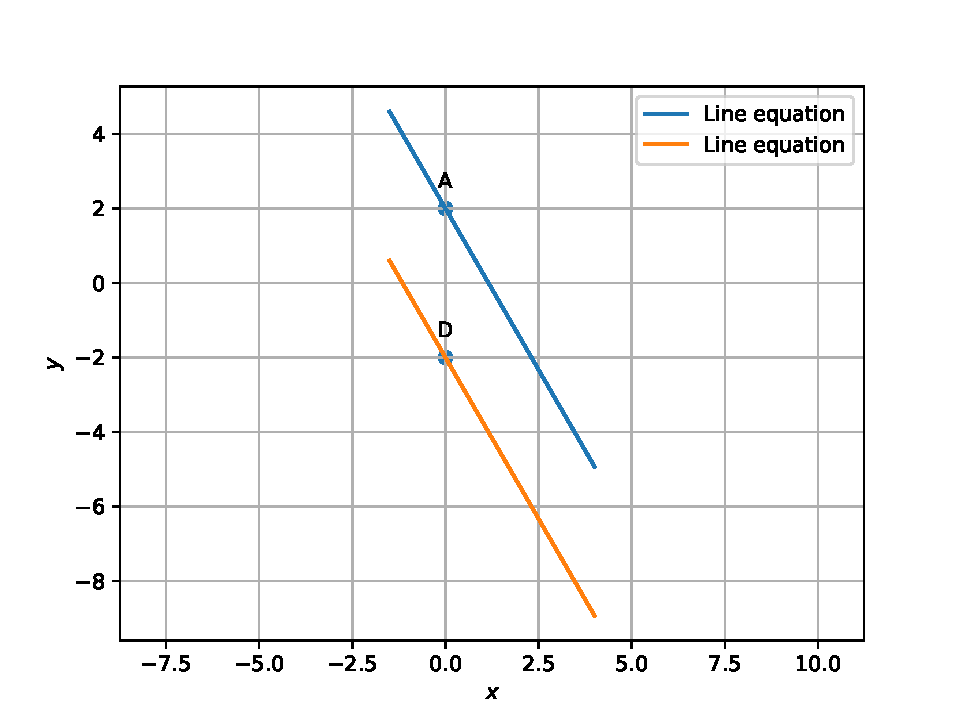
\includegraphics[width=\columnwidth]{chapters/11/10/2/14/figs/fig.pdf}
		\caption{}
		\label{fig:11/10/2/14}
  	\end{figure}
	\\
	\solution
\iffalse
	}

\section*{\large Solution}

\begin{figure}[H]
\centering
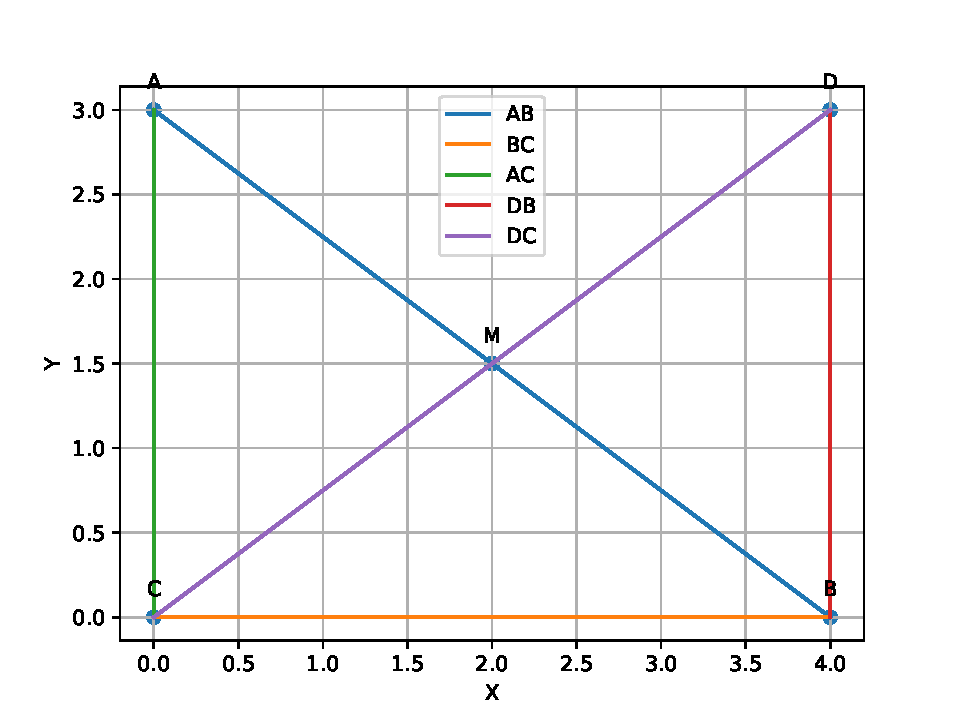
\includegraphics[width=1\columnwidth]{fig.pdf}
\caption{}
\end{figure}


\section{construction}

\begin{tabular}{|c|c|}
	\hline
	\textbf{Point}&\textbf{Value}\\
	\hline
	A&\myvec{0\\2}\\
	\hline
	$\theta$&2$\pi$/3\\
	\hline
	D&\myvec{0\\-2}\\
	\hline
	
	
\end{tabular}


\section*{Assumptions}
To find the line equation  through the point (0,2)
\vspace*{3mm}
\fi
From the  given information, the direction vector is
\begin{align}
	\vec{m}=\myvec{1\\-\sqrt{3}}
\end{align}
  
Thus, 
the normal vector is
\begin{align}
	\vec{n}=\myvec{\sqrt{3}\\1}
\end{align}

\iffalse
\begin{align}
	\vec{m}=\myvec{1\\-\sqrt{3}}
	\vec{n}=\myvec{\sqrt{3}\\1}
\end{align}


\begin{align}
	\vec{n^T}=(\sqrt{3}&1)	
\end{align}






Where line equation  is given by:
\begin{align}
\vec{n^T(x-p)}=0
\label{pf2-eq-1}
\end{align}

By substituting the values in the above equation:
\fi
and the 
equation of the line is 
\begin{align}
	\myvec{\sqrt{3} &1}\myvec{\vec{x}-\myvec{0\\2}}&=0
	\\
	\implies 
	\myvec{\sqrt{3}&1}
	\vec{x}&=2
\end{align}
The equation of the parallel crossing the Y-axis at a distance of 2 units below the origin is given by 
\begin{align}
	\myvec{\sqrt{3} &1}\myvec{\vec{x}-\myvec{0\\-2}}&=0
	\\
	\implies 
	\myvec{\sqrt{3}&1}
\vec{x}=-2
\end{align}

\item 
\label{chapters/11/10/2/15}
\iffalse
\documentclass[journal,10pt,twocolumn]{article}
\usepackage{graphicx, float}
\usepackage[margin=0.5in]{geometry}
\usepackage{amsmath, bm}
\usepackage{array}
\usepackage{booktabs}

\providecommand{\norm}[1]{\left\lVert#1\right\rVert}
\let\vec\mathbf
\newcommand{\myvec}[1]{\ensuremath{\begin{pmatrix}#1\end{pmatrix}}}
\newcommand{\mydet}[1]{\ensuremath{\begin{vmatrix}#1\end{vmatrix}}}

\title{\textbf{Line Assignment}}
\author{YOGEESH REDDY}
\date{September 2022}

\begin{document}

\maketitle
\paragraph{\textit{\large Problem Statement} -
\fi
The perpendicular from the origin to a line meets it at the point (-2,9). Find the equation of the line.
	\begin{figure}[!ht]
		\centering
 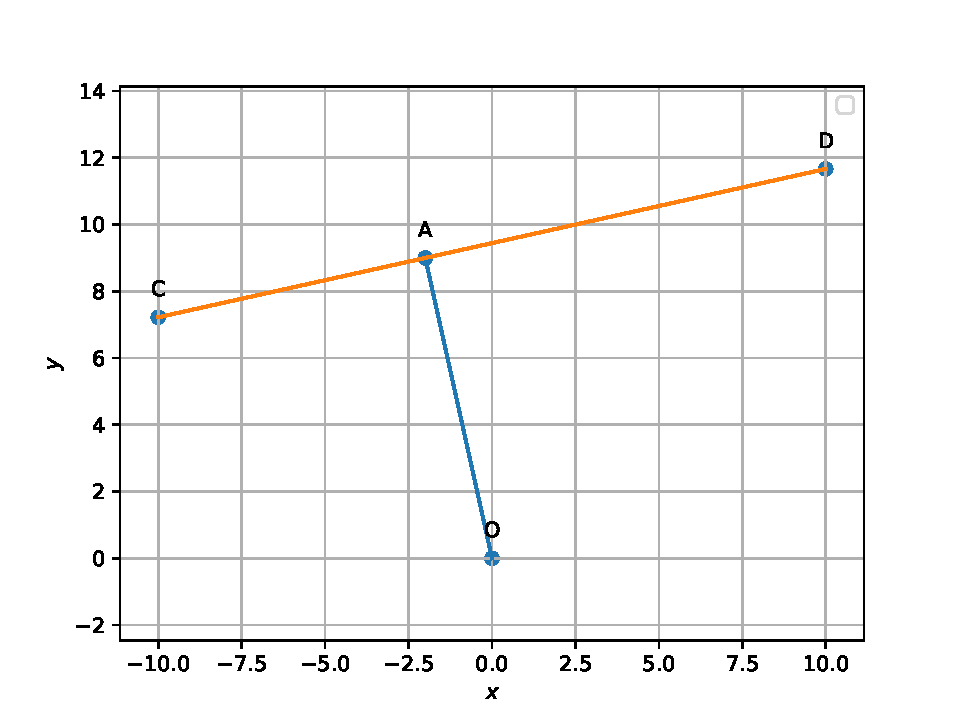
\includegraphics[width=\columnwidth]{chapters/11/10/2/15/figs/line.pdf}
		\caption{}
		\label{fig:11/10/2/15}
  	\end{figure}
	\\
	\solution
	\iffalse
\section*{\large Solution}
\begin{figure}[H]
\centering
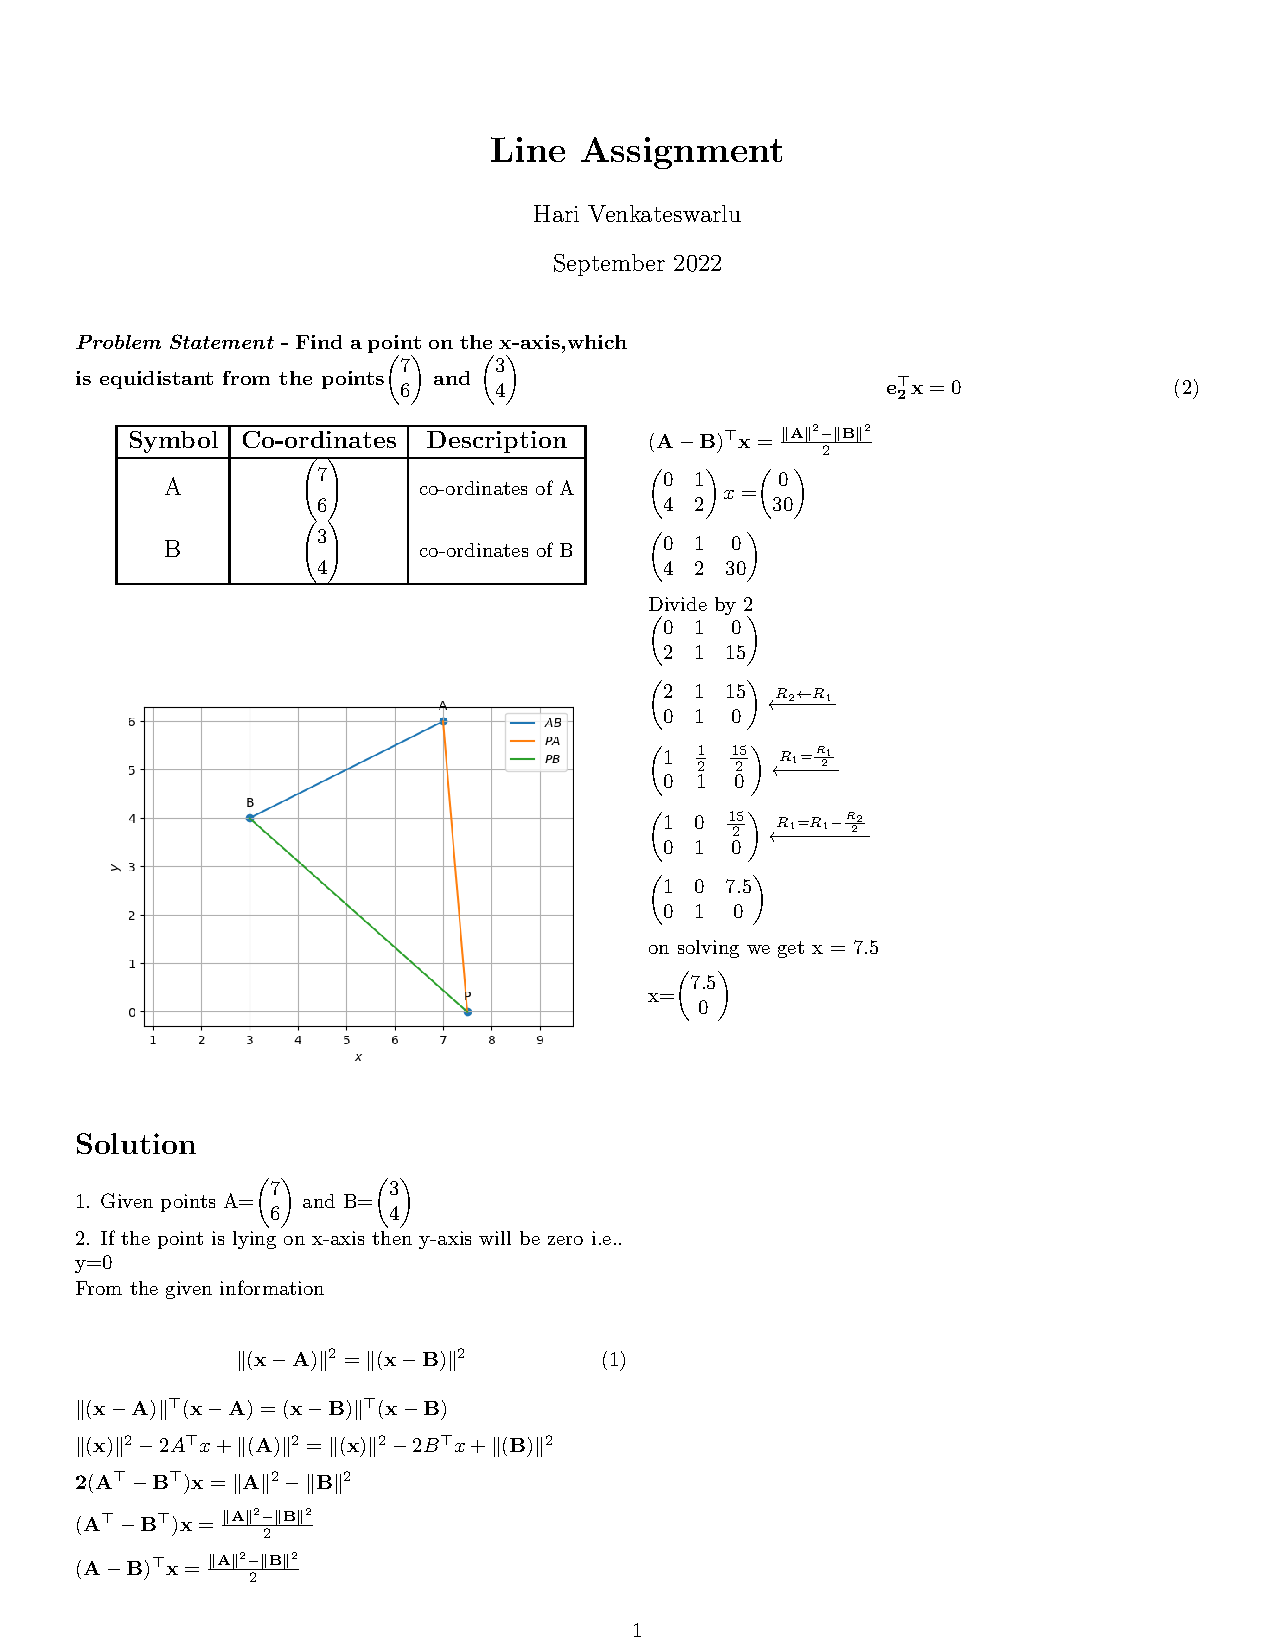
\includegraphics[width=1\columnwidth]{matrix.pdf}
\caption{}
\end{figure}

\section*{\large Construction}



The input parameters of figure 



\begin{table}[htbp]
 \begin{center}
    \begin{tabular}{|l|c|c|c|c|c|c} \hline \textbf{Symbol}
  & \textbf{value} \\
 \hline
O & $\myvec{0\\0}$ \\ \hline
A & $\myvec{-2\\9}$  \\ \hline
D &  $\myvec{x\\y}$  \\ \hline

 
\end{tabular}   
\end{center}
\caption{\label{table:dummytable} }
\end{table}

\vspace*{10mm}


\section*{Solution:}
\fi

Given 
\begin{align}
 \vec{0} = \myvec{0\\0},
 \vec{A} = \myvec{-2\\9}
\end{align}
\iffalse
Let D be a point on the required line :
\begin{align}
 \vec{D} = \myvec{x\\y}
\end{align} 
 \begin{align}
 \vec{D-A}=\myvec{x+2\\y-9}
   \end{align}
   \fi
   The 
normal vector is
\begin{align}
	\vec{n}&=\vec{O}- \vec{A}
	\\
	&=\myvec{2\\-9}
\end{align}
yielding the equation of the line as

\begin{align}
	\myvec{2 & -9}\brak{\vec{x} - \myvec{2 \\ -9}}&= 0
	\\
	\implies 
	\myvec{2 & -9}\vec{x} &= 85
\end{align}
\iffalse

\begin{align}
 2\vec{x}-9\vec{y}+85=0
\end{align}


\end{document}
\fi

\item 
\item 
\item 
\item 
\item 
\label{chapters/11/10/2/20}
\iffalse
\def\mytitle{MATRICES USING PYTHON}
\def\myauthor{R.Ramesh}
\def\contact{rameshrandhiglra@gmail.com}
\def\mymodule{Future Wireless Communication (FWC)}
\documentclass[10pt, a4paper]{article}
\usepackage[a4paper,outer=1.5cm,inner=1.5cm,top=1.75cm,bottom=1.5cm]{geometry}
\twocolumn
\usepackage{graphicx}
\graphicspath{{./images/}}
\usepackage[colorlinks,linkcolor={black},citecolor={blue!80!black},urlcolor={blue!80!black}]{hyperref}
\usepackage[parfill]{parskip}
\usepackage{lmodern}
\usepackage{tikz}
	\usepackage{physics}
%\documentclass[tikz, border=2mm]{standalone}
\usepackage{karnaugh-map}
%\documentclass{article}
\providecommand{\sbrak}[1]{\ensuremath{{}\left.#1\right]}}
\usepackage{tabularx}
\usepackage{circuitikz}
\usetikzlibrary{calc}
\usepackage{amssymb,amsfonts,amsthm,amsmath}
\newcommand{\myvec}[1]{\ensuremath{\begin{pmatrix}#1\end{pmatrix}}}
\usepackage{amssymb}
\renewcommand*\familydefault{\sfdefault}
\usepackage{watermark}
\usepackage{lipsum}
\usepackage{xcolor}
\usepackage{listings}
\usepackage{float}
\usepackage{titlesec}
\usepackage{amssymb,amsfonts,amsthm,amsmath}
\usepackage{cite}
\usepackage{amssymb,amsfonts,amsthm,amsmath}
\usepackage{algorithmic}
\usepackage{graphicx}
\usepackage{textcomp}
\usepackage{xcolor}
\usepackage{txfonts}
\usepackage{listings}
\usepackage{enumitem}
\usepackage{mathtools}
\usepackage{gensymb}
\usepackage{bm}
\usepackage{polynom}

\providecommand{\res}[1]{\Res\displaylimits_{#1}} 
%\providecommand{\norm}[1]{\lVert#1\rVert}
\providecommand{\mtx}[1]{\mathbf{#1}}
\providecommand{\fourier}{\overset{\mathcal{F}}{ \rightleftharpoons}}
%\providecommand{\hilbert}{\overset{\mathcal{H}}{ \rightleftharpoons}}
\providecommand{\system}{\overset{\mathcal{H}}{ \longleftrightarrow}}
	%\newcommand{\solution}[2]{\textbf{Solution:}{#1}}
\newcommand{\solution}{\noindent \textbf{Solution: }}
\newcommand{\cosec}{\,\text{cosec}\,}
\newcommand{\mydet}[1]{\ensuremath{\begin{vmatrix}#1\end{vmatrix}}}
	\newcommand*{\permcomb}[4][0mu]{{{}^{#3}\mkern#1#2_{#4}}}
\newcommand*{\perm}[1][-3mu]{\permcomb[#1]{P}}
\newcommand*{\comb}[1][-1mu]{\permcomb[#1]{C}}
\providecommand{\fourier}{\overset{\mathcal{F}}{ \rightleftharpoons}}
%\providecommand{\hilbert}{\overset{\mathcal{H}}{ \rightleftharpoons}}
\providecommand{\system}{\overset{\mathcal{H}}{ \longleftrightarrow}}
\providecommand{\mtx}[1]{\mathbf{#1}}
\titlespacing{\subsection}{1pt}{\parskip}{3pt}
\titlespacing{\subsubsection}{0pt}{\parskip}{-\parskip}
\titlespacing{\paragraph}{0pt}{\parskip}{\parskip}
\newcommand{\figuremacro}[5]{
    \begin{figure}[#1]
        \centering
        \includegraphics[width=#5\columnwidth]{#2}
        \caption[#3]{\textbf{#3}#4}
        \label{fig:#2}
    \end{figure}
}

\let\vec\mathbf
\lstset{
frame=single, 
breaklines=true,
columns=fullflexible
}
%\thiswatermark{\centering \put(0,-90.0){\includegraphics[scale=0.5]{iit h.png}} }
\title{\mytitle}
\author{\myauthor\hspace{1em}\\\contact\\FWC22076\hspace{6.5em}IITH\hspace{0.5em}\mymodule\hspace{6em}September}
\date{}


\begin{document}
\maketitle
\paragraph{\textit{\large Problem statement: }\\
\fi
 By using the concept of equation of a line, prove that the three points (3, 0), (– 2, – 2) and (8, 2) are collinear.
	\begin{figure}[!ht]
		\centering
 \includegraphics[width=\columnwidth]{chapters/11/10/2/20/figs/figs6.pdf}
		\caption{}
		\label{fig:11/10/2/20}
  	\end{figure}
	\\
	\solution 
 \iffalse
 \section*{Construction}
 	\begin{center}
\textsl{}  \includegraphics[scale=0.49]{figs6.pdf}
  
  Figure of construction
  	\end{center}
The input parameters for this construction are 
\begin{center}
\begin{tabular}{|c|c|c|}
	\hline
	\textbf{Symbol}&\textbf{Value}&\textbf{Description}\\
	\hline
	$\vec{A}$&\myvec{3\\0}&collinear point\\[8pt]
	\hline
		$\vec{B}$&\myvec{-2\\-2}&collinear point\\[8pt]
	\hline
		$\vec{C}$&\myvec{8\\2}&collinear point\\[8pt]
	\hline

\end{tabular}
\end{center}
\section*{Solution}
\textbf{Statement:}
the rank of matrix defines number of linearly dependent vectors.  
\\

\begin{align}
	  \vec{D}= \vec{A}- \vec{B}
	  \\
	  = {\myvec{ 3 \\ 0}-\myvec{-2 \\ -2}}
	  \\
	  =\myvec{-5 \\ -2}
 \end{align}
  \begin{align}
	  \vec{E}= \vec{A}- \vec{C}
	  \\
	  ={\myvec{ 8 \\ 2}-\myvec{3 \\ 0}}
	  \\
	  =\myvec{ 5 \\ 2}
  \end{align}
   Now the matrix is:
\begin{equation}
\boldsymbol{F}=
\begin{pmatrix}
 
     \boldsymbol{D} & \boldsymbol{E}
 \end{pmatrix}
 \end{equation}
 \fi
 The collinearity matrix can be expressed as
 \begin{align}
			    \myvec{-5 & -2
			    \\
			    5 & 2 }  
			    \xleftrightarrow[]{R_2 \leftarrow {R_1 + R_2}}
			   = \myvec{	    -5 & -2  
			    \\
			    0 & 0}  
\end{align}
which is a rank 1 matrix.
\iffalse
\textbf{}From the above rank of matrix is 1
\\
\textbf{If rank of matrix F is "1"  then the vectors  are in linearly dependent.so points are in collinear.} 
  
\end{document}
\fi


\end{enumerate}
